\chapter{Electron diffraction in an imperfect crystal -- TKD}
\label{chap:TKD}
% Context
In the previous chapters we have established that the electron channelling (diffraction) contrast  technique in the scanning electron microscope is a great tool to investigate dislocations close to a surface in crystalline materials. In this chapter we will explore different diffraction techniques used for the study of different kind of crystal imperfections. 



So far, we have focused mostly on elastic, coherent scattering. We treated inelastic scattering as a channel of intensity loss in the diffraction beams and approximated its effect through the complex optical crystal potential. Since Kikuchi patterns are not only formed by electrons of incident energy, we need to take a closer look, on page~\pageref{sec:scatter}, at models used to predict energy loss for high energy electrons.


While the physics of EBSD is somewhat well understood, the question explored in this chapter is whether the existing models can accommodate for the new geometry of the transmission-EBSD modality. In the following pages the implementation of diffraction pattern predictions of EMsoft software~\cite{EMsoftpaper} is described (page~\pageref{sec:TKDtheory}). Then, I will talk about the difference in electron escape distances between the EBSD and TKD modalities, as predicted by Monte Carlo simulations, and why that matters on page~\pageref{sec:MC}. 


The work I will show in this chapter was the outcome of a collaboration with Prof. Marc De Graef's group and parts of the results were published in \textit{Energy-weighted dynamical scattering simulations of electron diffraction modalities in the scanning electron microscope}~\cite{PascalTKD}.

%Outline
In section~\ref{sec:TKDtheory} on page~\pageref{sec:TKDtheory} we describe the typical geometries for EBSD, TKD and ECP data acquisition and formulate a general expression for the thickness integrated back-scattered electron intensity that is applicable to all three diffraction modalities. We describe the particulars of the Monte Carlo trajectory simulations in section~\ref{sec:MC}, along with the resulting differences between the modalities. Master patterns for the three modalities are described and compared in section~\ref{sec:comparison}. 



%%%%%
\section{Introduction}


\subsection{How does it work?}
\label{sec:EBSD}

Let us cover the grounds of the technique first. What we need for an electron backscatter pattern (EBSP) is a sample with a flat surface placed at a shallow angle of about \SI{20}{\degree} with respect to the incident electron  beam as schematically shown in Fig.~\ref{fig:geometries} a). The location where the \SIrange{10}{30}{\kilo \electronvolt} stationary beam is incident on  the sample surface also marks the source of the spherically generated EBSD pattern. 

\begin{figure}[ht]
\centering
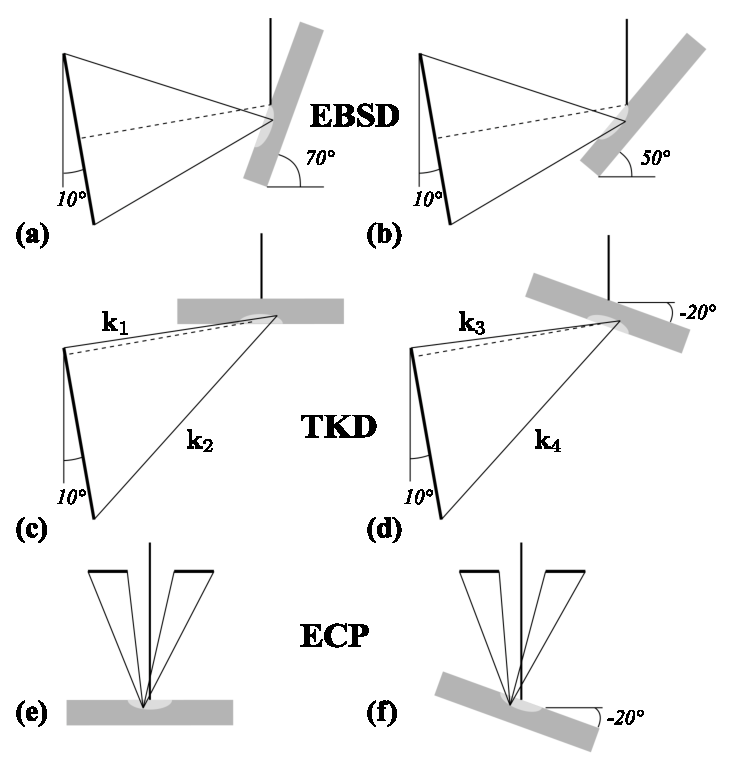
\includegraphics[width=0.6\linewidth]{Fig3.eps}
\caption[EBSD, TKD and ECP set-up geometry.]{(a) and (b) EBSD geometry, with the sample inclined at $70^{\circ}$ and $50^{\circ}$; the detector is indicated by a thick line and is inclined by $10^{\circ}$ with respect to the vertical direction. (c) and (d) show typical TKD geometries with a horizontal sample, and one inclined at $-20^{\circ}$. (e) and (f) show typical ECP geometries with two different sample tilt angles.  Adapted from \cite{PascalTKD}.}
\label{fig:geometries}
\end{figure}

An example of this is shown in Fig.~\ref{fig:tkspatter} for a 20 keV electron beam incident on a Ni sample. The simulation was done using EMsoft~\cite{EMsoft} and shows all possible independent exit directions in the Northern hemisphere as a stereographic projection (see ref.~\cite{degraef2013e}). 

\begin{figure}[ht]
\centering
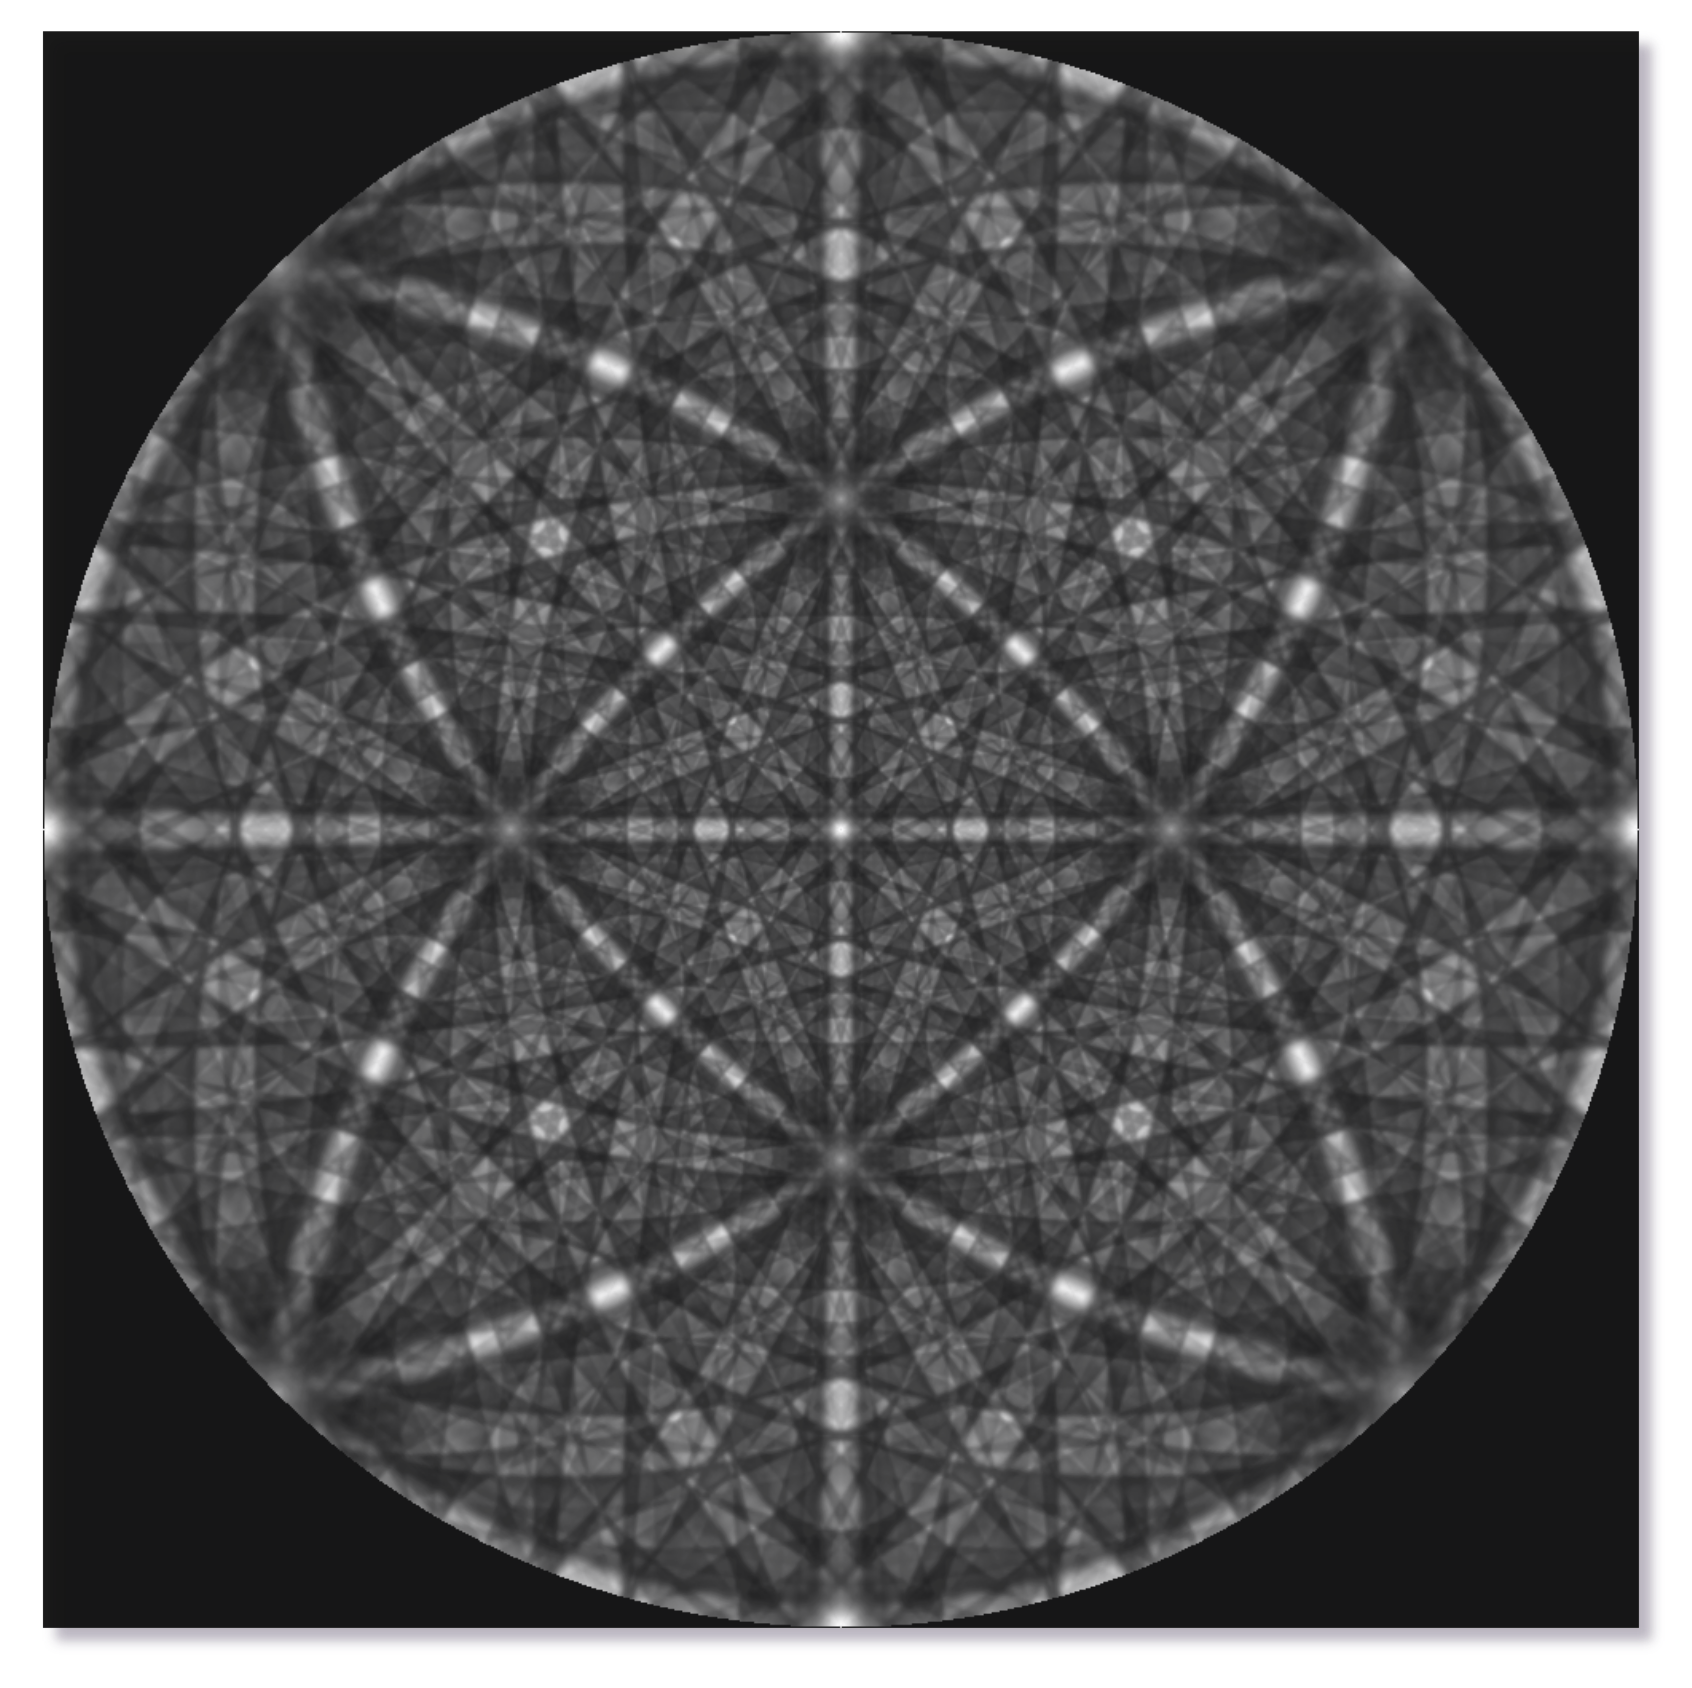
\includegraphics[width=0.7\linewidth]{TKDpattern.png}
\caption[EBSD pattern of Ni northern hemisphere.]{Simulated stereographic projection of the entire Northern hemisphere  EBSD pattern of Ni using 20 keV incident electrons. The 90$^{\circ}$ represents the north pole and the 0$^{\circ}$ circle the equator and the geometry of the crystal is shown in the bottom left corner (see also Fig. \ref{fig:TKDgeometry} for coordinate frames geometry). The blue rectangle shows the area plotted in Fig.  \ref{fig:MPs}. Adapted from \cite{PascalTKD}.}
\label{fig:tkspatter}
\end{figure}


Primary beam electrons that have lost little energy on their way in the sample, have a chance to suffer diffraction at crystal planes on their way out of the sample. The Kikuchi lines in the EBSD pattern tell us about the crystal planes in the sample we are probing with the electron beam. 


 If a phosphorous screen is placed close to the sample, on the path of the diffracting out electrons, then we can record a small solid angle of the pattern shown here. Nevertheless, with the help of careful analysis it will provide enough information to learn about the crystallography of this sample. 
 
 For a polycrystalline sample, using the scanning setting of the SEM one could record  EBSD patterns for every single pixel and then analyse them to obtain texture information, misorientation or strain variation from one grain to the other.  Automated pattern indexing software established this diffraction modality as one of the conventional tools of orientation mapping, phase identification and/or relative lattice strain estimation in crystalline materials \cite{schwartz2009a}. A better descriptions of this can be found in textbooks such as Chapter 2 in~\cite{Maitland07}.



%%%%
\subsection{Kikuchi patterns -- three ways}
\label{sec:Kikuchi}





%EBSD/TKD - channelling out
We can distinguish a number of different SEM modalities making use of the Kikuchi diffraction mechanism. If the recorded electrons are the backscattered ones (see Fig.~\ref{fig:geometries} a), b)), then the technique is known as electron backscatter diffraction (EBSD) and the Kikuchi patterns obtained are called electron backscatter patterns (EBSP).  In order to increase the diffraction signal in this mode, the popular approach has been to tilt the sample to about $70^{\circ}$ from horizontal towards the detector, which guarantees a maximum backscattered electron yield. However, the high tilt will also spread out the information volume (or interaction volume) of the electrons within the sample, limiting the achievable spatial resolution.


The idea of questioning instead the electrons transmitted through a thin sample for diffraction information, as a method of improving the lateral spatial resolution, has attracted considerable attention in recent years~\cite{Trimby12,Keller12}. In this case the detector is placed on the other side of a thin sample and transmission Kikuchi diffraction patterns are collected as seen in Fig.~\ref{fig:geometries} c) and d).


%ECP - channelling in
The modalities above are sometimes referred to as ``channelling out'' diffraction techniques~\cite{joy1994} to suggest that the diffraction information has been sampled by electrons on their way out of the sample and that the volume from which the signal is collected is located close to the exit surface. The SEM can also be used in ``channelling in'' mode when electron channelling patterns (ECPs) are acquired~\cite{Coates67,Joy82}. The usual set-up  geometry is shown in Fig.~\ref{fig:geometries} e) and f). In this case, Kikuchi-like diffraction patterns can also be obtained by varying the incident beam direction with respect to the crystal. Typically, those patterns have a smaller solid angle compared to their EBSD counterparts. Nevertheless, the physical scattering mechanisms that produce EBSPs and ECPs are related through the reciprocity principle~\cite{reimerSEM}.

\subsection{Interaction volume}


\begin{sidewaysfigure}
\centering
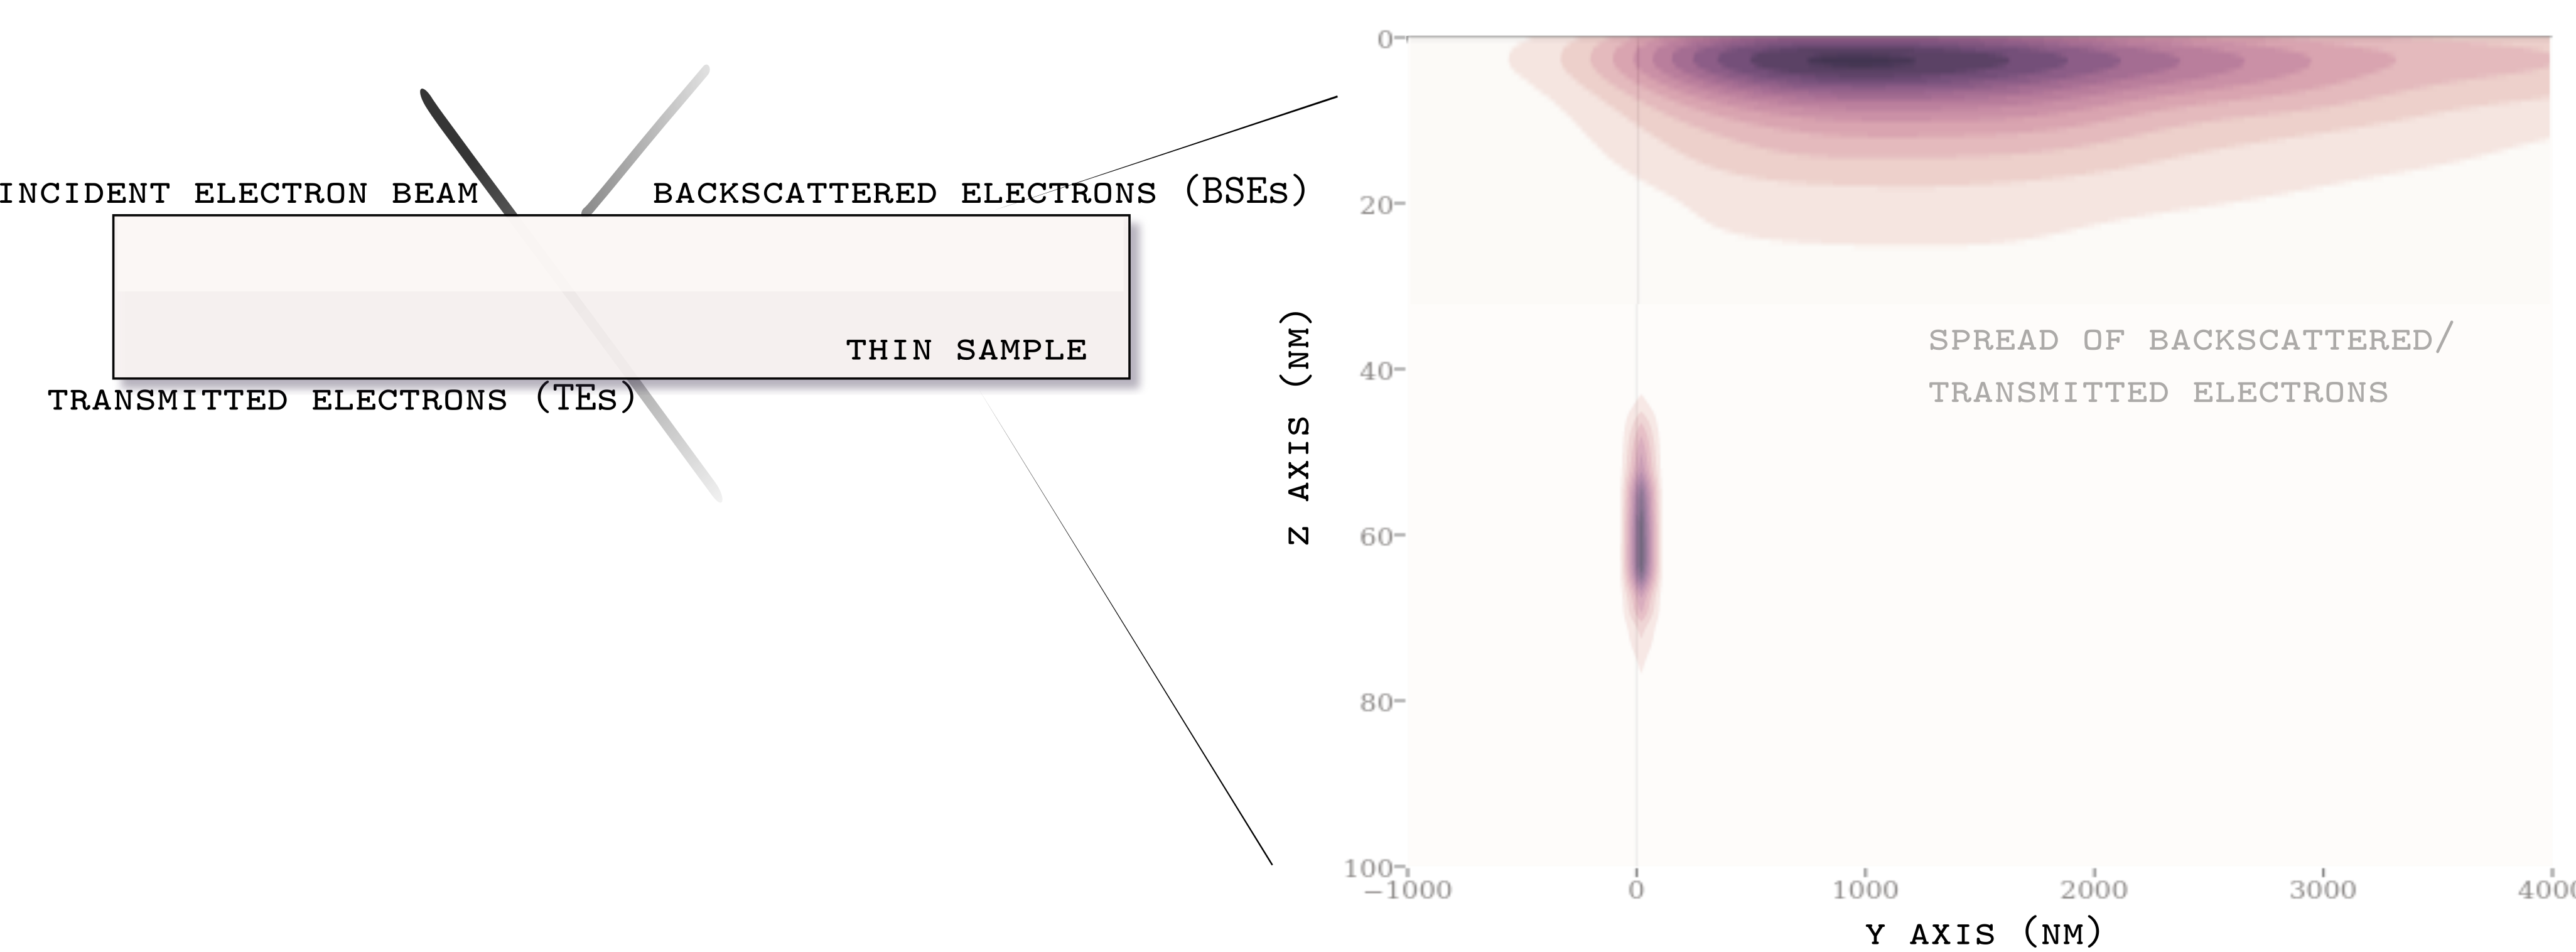
\includegraphics[width=0.9\linewidth]{Figures/TKDpendepth.png}
\caption[Interaction volume]{Interaction volume of backscattered (top images) and transmitted electrons (bottom images) shown here as kernel density estimates plots of the escaping electrons. The darker colour indicates larger probability of large angle elastic scattering event in that region.}
\label{fig:intvolume}
\end{sidewaysfigure}



As a SEM based technique, EBSD is limited in its spatial resolution by the SEM electron optics. When we talk of high resolution imaging of nano-grains, we imply the use of a high performance FE-SEM, short working distances, which in turns require small samples and small interaction volumes. We will see on page~\pageref{sec:motivation} that the latter argument motivates the need for the transmission mode of EBSD, namely transmission-EBSD or transmission Kikuchi diffraction (TKD). In conventional EBSD geometry the signal carrying electrons are the backscattered ones. These are electrons which can travel a significant distance before escaping the sample, ``sampling'' a rather broad interaction volume. 



The difference in interaction volume is shown in Fig.~\ref{fig:intvolume} as KDE plots~\cite{KDE}. The position of escaping electrons is assumed to be the last scattering event before exiting the sample.  The data was produced from Monte Carlo simulations using Casino~\cite{casino} software for an incident beam of 30 keV on a \SI{70}{\degree}~(EBSD -- top figure) and a \SI{20}{\degree}~(TKD -- bottom figure) tilted sample of thin Si. I used different sample thicknesses in order to produce the same total number of backscattered and transmitted electrons. More about the description of the Monte Carlo method used on page~\pageref{sec:MC}.







\subsection{TKD geometry}

Following the EBSD experimental geometry described by Callahan~\cite{degraef2013e} we can derive the TKD sample-detector coordinates transformation.


\noindent \begin{minipage}{0.55\textwidth}
\vspace{0.5cm}
For a translation vector $\textbf{t}$ which moves the origin of the detector frame $O_d$ to the origin of the sample frame $O_s$ defined as:
\begin{equation*}
    \vec{t}=(x_{PC}, y_{PC}, L),
\end{equation*}
the coordinates of a point $P(x_P, y_P)$ on the detector in the reference frame of the sample can be derived geometrically:
\begin{equation*}
   \vec{O_sP} = \mathcal{R}^{ds}(\vec{O_dP} -\vec{t})
\end{equation*}
where   $\mathcal{R}^{ds}$    is the coordinate transformation from the sample frame to the detector frame. Such that finally the direction cosines of a pixel on the screen in the sample frame is:
\begin{equation*}
    P^s=\begin{pmatrix}
    -\cos{\alpha}(y_d-y_{PC}) + L \sin{\alpha}   \\
    -(x_{PC}-x_d)\\
    -\sin{\alpha}(y_d-y_{PC}) + \cos{\alpha}(z_d-L)  
    \end{pmatrix}, 
\end{equation*}
\begin{equation*}
     \, \text{where} \,\alpha =\pi/2 + \theta_S + \theta_D.   
\end{equation*}    
\end{minipage}
\begin{minipage}{0.45\textwidth}
    \centering
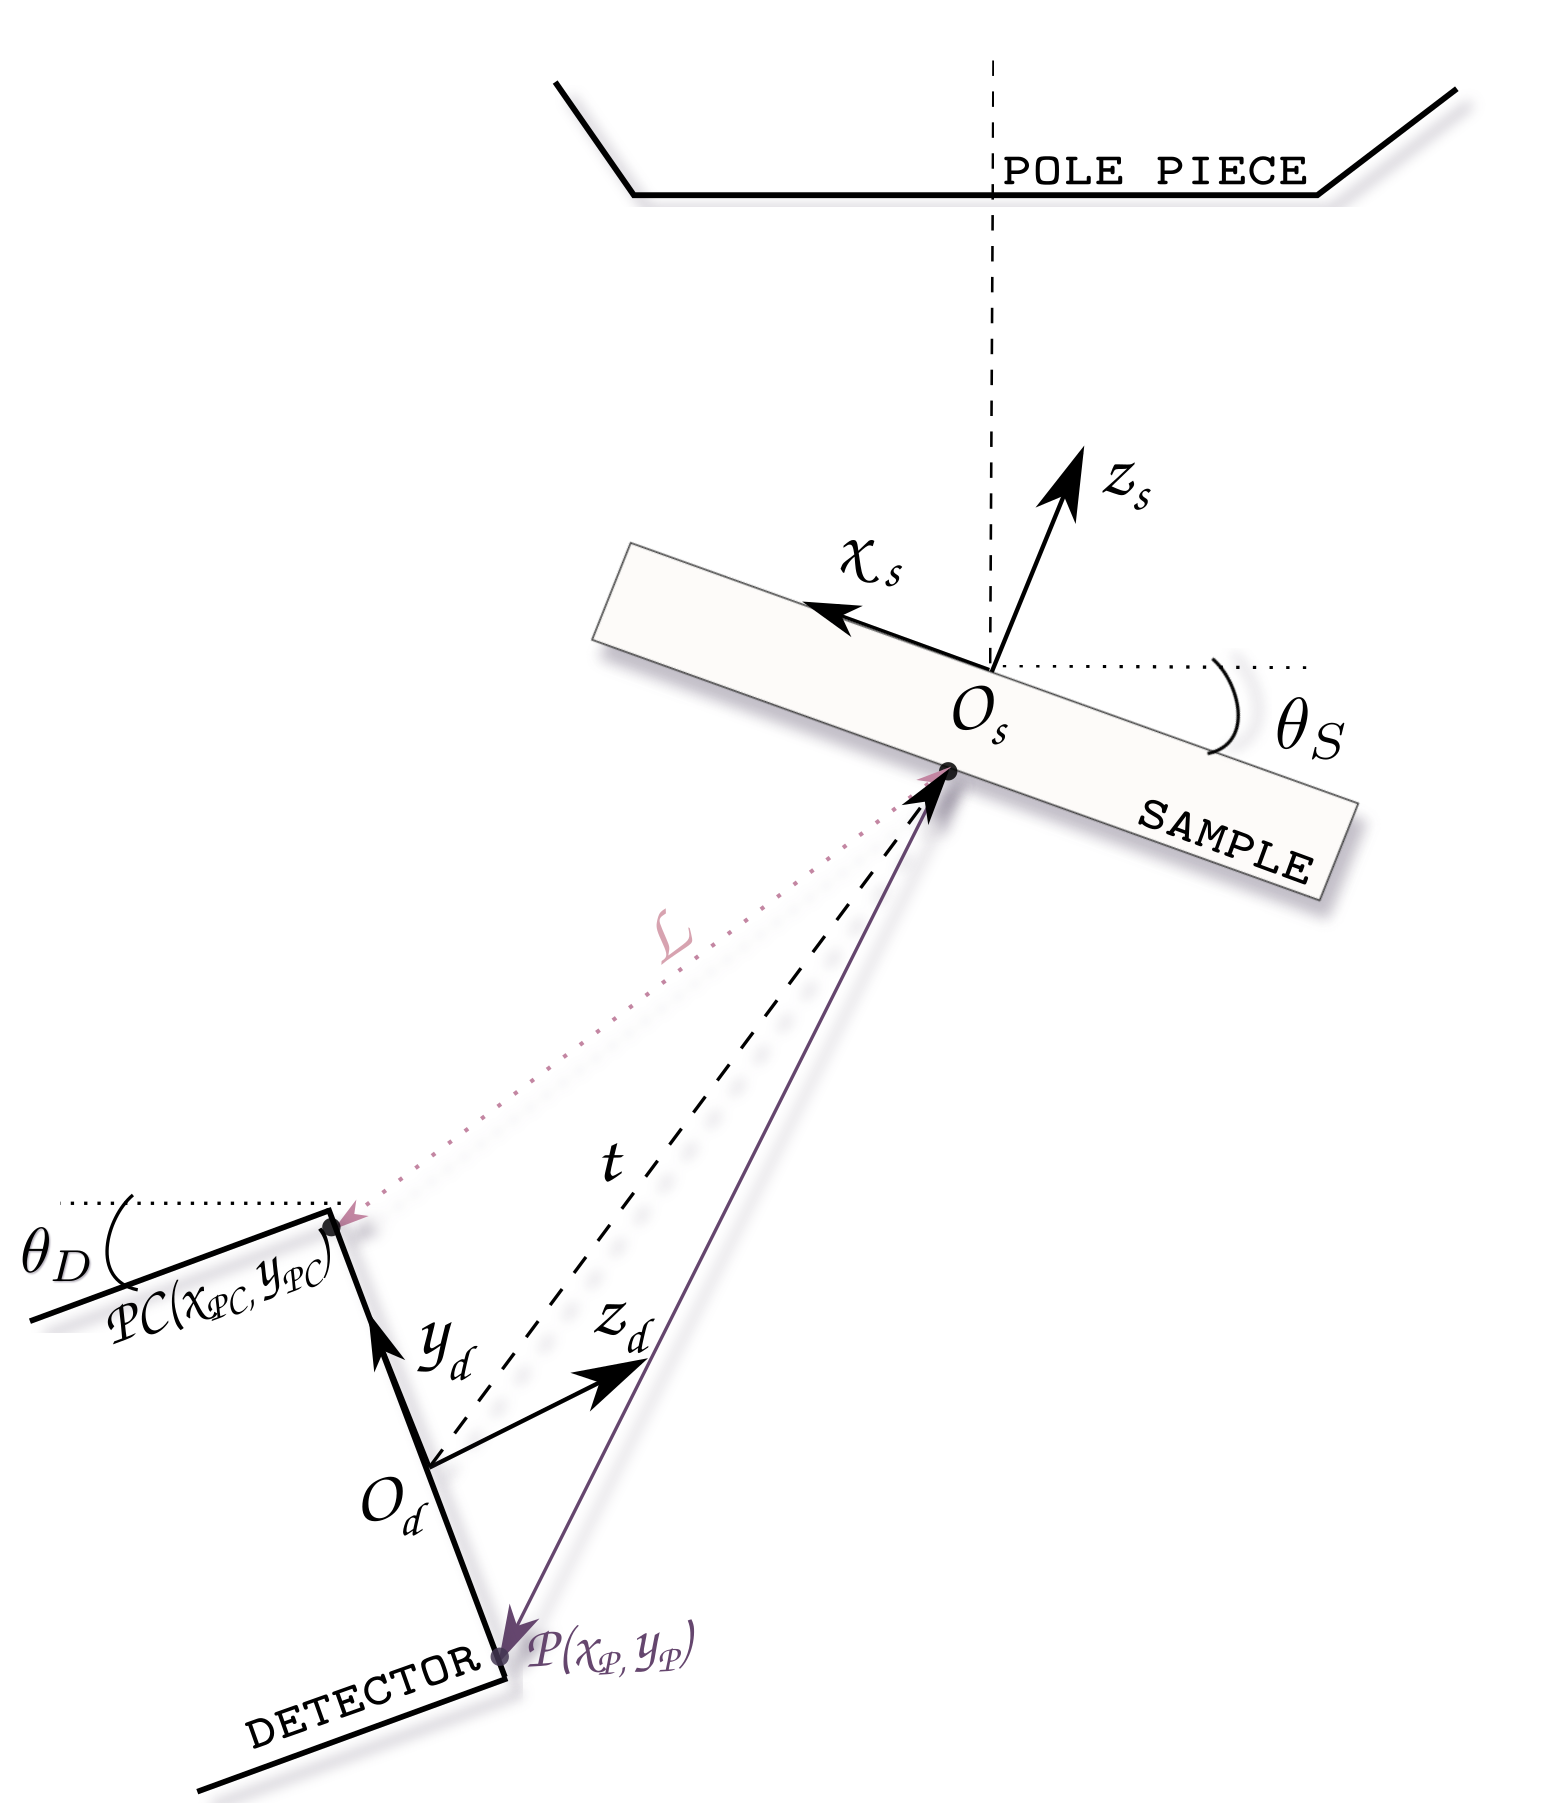
\includegraphics[width=1.15\linewidth]{TKD_geom.png}
\captionsetup{width=0.7\linewidth}
\captionof{figure}[Schematics of TKD set-up geometry]{Schematics of TKD set-up geometry. PC denotes the pattern centre and L is the distance between the detector and the sample.} 
\label{fig:TKDgeometry}
\end{minipage}

\vspace{0.3cm}


For a given crystallographic orientation the direction cosines can be converted to the possible channelling out directions the pixels on a detector will register. This can be done for all grains in a sample and the information  can be stored in a look up table.






%%%%
\subsection{Why do we need a new model?}
\label{sec:motivation}


%Why
The geometry of the Kikuchi patterns is dictated by the unit cell of the crystal and its orientation. Other features, such as the width of the bands, for instance, are nevertheless influenced by the spatial distribution of diffracted electrons in the sample and their energy distribution. In the end, Kikuchi patterns offer a variety of information about the crystal structure of the material under investigation which is why they are widely used in the study of new materials. For a more complete discussion see ref.~\cite{winkelmann2017}.


% Gap
Theoretical models have been developed and successfully applied to retrieve this wealth of information by taking into account the full dynamical behaviour of electron diffraction~\cite{Winkelmann07, Picard14, singh2016}. Electron diffraction calculations commonly handle inelastic scattering in a phenomenological way through the introduction of a complex optical crystal potential approximation. This assumption implies that inelastically scattered electrons, once they lose even a small amount of energy, will cease to contribute to the diffraction pattern. The predicted diffraction patterns based on this simplified model remain meaningful~\cite{howie1963} but, understandably, are lacking quantitative precision. Due to the strong interaction of incident beam electrons at SEM energies with matter, the inelastic cross section is always comparable to the elastic one, and a portion of inelastically scattered electrons will reach the detector and contributes to the imaged pattern. 

Depending on the types of inelastic channels allowed, these electrons can suffer diffraction after losing a small amount of energy, contributing then to the diffuseness of the Kikuchi patterns. This process is especially relevant for ``channelling out'' modalities where electrons with energies lower than the incident energy can still contribute to the diffraction pattern. Alternatively, if electrons are scattered at a large angle multiple times such that memory of their original direction is lost, they will also contribute to the background intensity. This is the case for both channelling modalities. We call the later type of inelastically (back/forward-)scattered electrons (B/F)SE2 in order to differentiate them from (B/F)SE1 electrons carrying diffraction information.

It is therefore essential to explicitly consider inelastic scattering and its effects on the signal contributing electrons, such as their energy and spatial distributions~\cite{degraef2013e, winkelmann2016}. This is especially important if finer features of the Kikuchi bands (size, absolute intensity relative to background, band edges) are to be correctly predicted. A full account of the inelastic channels in electron diffraction poses a challenging problem. While general Schr\"odinger equation solutions for inelastic scattering in perfect crystals have been proposed by Yoshioka~\cite{yoshioka1957a} and solved for various electron microscopy applications (see Howie~\cite{howie1963} for small angle plasmon scattering and Forbes et al.~\cite{forbes2011} for single thermal diffuse scattering events), to our knowledge, readily implementable solutions relevant for SEM electron energies have yet to be proposed.

% Solution
In this work, we assume inelastic scattering events to be stochastic and that Monte Carlo (MC) technique can estimate both the trajectories of electrons that suffered such events as well as their energy distribution. Such models have been proposed and widely used to correctly predict distributions of backscattered electrons~\cite{joy1995a}. The assumption that the distribution of escape energies and the trajectories of electrons carrying diffraction information can be estimated from the last elastic event predicted by MC models has already been successfully applied both for EBSPs~\cite{degraef2013e} and ECPs~\cite{degraef2017k}. 

The energy of the electron at the last elastic event before escaping the sample, is considered to be the energy for which the diffraction occurs. Similarly, the distance to the exit surface from the last elastic event, also known as the escape or exit distance, is used as the diffraction distance (electron path length over which coherence is not lost). Dynamical diffraction modelling is then applied for the full MC predicted electron energy and path distributions. Here, we extend this model to TKD patterns by considering the geometry of a thin film sample where the entry (top) and escape (bottom) surfaces are different such that the incoherent events acting as sources of diffracting electrons are scattering in a forward direction. 

While this approach may not take into account the full extent of inelastic scattering effects on diffracted electrons proposed by the Yoshioka equations, it leads to a model of manageable complexity which is straightforward to implement and whose predictions are easily understood. Most importantly, it represents a step forward in taking into account the full physics of electron diffraction in matter by considering the full distribution of energies of channelling electrons and produces accurate predictions when compared to experimental patterns, as shown in section~\ref{sec:comparison} on page~\pageref{sec:comparison}.


%%%%%%%%%%%
\subsection{Electron scattering}
\label{sec:scatter}

So far we have only talked about one type of electron scattering: the coherent, elastic type that is also known as diffraction. But electrons can scatter in a variety of ways.  Classically, the collision of particles is fully defined by their velocities and interaction parameters. However, high energy electrons are quantum mechanical objects. The notion of defined path for a particle with known velocity is meaningless in the Copenhagen interpretation of the quantum mechanical world\footnote{Note that in the Bohmian interpretation this is allowed \cite{Cheng18}.}. In any interpretation of quantum mechanics a version of the uncertainty principle limits us from knowing both the precise position and velocity of a particle, making the classical approach of predicting particle behaviour unfeasible at the scale of the very small. Instead, we are interested in defining the probability that, as a result of the collision, the particle will deviate by a given angle. This is what we mean by \textit{scattering}.

For practical considerations it is common to classify the interaction of electrons with a crystal in two distinct processes:
\begin{itemize}
\item \textit{Elastic scattering}, defined as a process which does not change the state of the crystal. Mostly made up by interactions with the nucleus. \textit{Rutherford scattering} is the model commonly used to predict this behaviour and it does that by taking into account just Coulomb forces between the charged electron and the nucleus. 

Let's say an elastic event will deviate the trajectory of an electron by a polar angle $\phi$ from its original trajectory. The probability of the electron being scattered in the solid angle ${d \Omega}$ is given by the angular differential form of the screeened Rutherford cross section~\cite{Reimer76}:
\begin{equation*}
\frac{d \sigma}{d \Omega} = \left( \frac{e^2 }{4 \pi \epsilon_0 } \frac{Z}{4 E}\right)^2 \frac{1}{\sin^2{\frac{\phi}{2}} + \alpha} (\si{m^{-2}})
\end{equation*}

where $E$ is the energy of the electron in \si{\kilo eV}and $\alpha$ is a screening factor accounting for the fact that some of the atomic charge is ``screened'' by the orbiting electrons from the perspective of the incident electrons.

As a result, it is common to assume that this scattering mechanism accounts for  the bulk of angular scattering of electrons including the behaviour we call backscattering.


\item \textit{Inelastic scattering}, defined as the process in which the state of the crystal is modified by the interaction. An important contribution here is made by the electron-electron scattering which causes the incident beam electron to loose small amounts of energy to the crystal. The angular deflections caused by these events is relatively small allowing us to use, what is known as, the \textit{continuously slowing down approximation} (CSDA) to  predict this particular type of inelastic scattering processes. We simply assume the electrons are carrying on the same path but slowly and continuously lose energy. The \textit{Bethe's theory} describes electrons as a system of oscillators that lose energy due to excitations caused by the crystal and can predict a \textit{stopping power} of inelastic events~\cite{joy1989}:
\begin{equation}
    \frac{dE}{ds} = -2\pi e^4 N_A  \frac{Z \rho}{A E} \log{\left( \frac{1.166E}{J}\right)} \, \, \, (\si{eV/\angstrom})
\end{equation}
where $E$ is the incident energy in units of \si{\eV}, $s$ is the path length along the trajectory (in \si{\angstrom}), $N_A$ is Avogadro's number, $\rho$ is the density (in \si{\gram/\cm^3}), $Z$ is the atomic number and $A$ is the atomic weight of the target. $J$ is an empirical parameter representing the mean ionisation potential, has units of \si{\eV} and represents the effective average energy loss of the incident electron in the material. $\pi e^4$ is a common constant appearing in inelastic scattering cross sections and used in Gaussian units:
\begin{equation*}
\pi e^4 = \pi (a_0 E_h) (\si{\cm^2 \eV^2})
\end{equation*}
where $a_0$ is the Bohr radius and  $E_h$ is the Hartree constant. The pre-multiplying factors are sometimes written out explicitly as:
\begin{equation}
    2 \pi e^4 N_A = 784 (\si{\eV^2 \cm \angstrom/  \mol) }.
\end{equation}
\end{itemize}


In order to predict the probability of electrons scattering in a certain direction and reach a certain energy, one has to combine the two scattering processes. When it comes to probability prediction, Monte Carlo methods are the answer as we will see on page~\pageref{sec:MC}.





%%%%
\section{Theoretical Model}
\label{sec:TKDtheory}

This section will review the energy weighted dynamical theory implemented by EMsoft~\cite{EMsoft}.

%
\subsection{Energy and diffraction distance integrated electron intensity}
\label{sec:energy_weight}


The simulation of the (back/forward-)scattered electron distribution emerging from a sample illuminated with a fine, nearly-parallel, electron probe can be achieved in general by integrating over both the energy range of the exiting electrons and the distance travelled in the sample between the scattering site and the sample surface. The probability of a (B/F)SE emerging from the sample in the direction $\hat{\mathbf{k}}$ (the hat indicates a unit vector) can be written as follows:
\begin{equation}
    P(\hat{\mathbf{k}}) = \sum_{n\in\text{A.U.}} P_n(\hat{\mathbf{k}}),
\end{equation}
where A.U. stands for asymmetric (primitive) unit and the index $n$ runs over all positions in the asymmetric unit.  The probability $P_n$ is defined as:
\begin{equation}
    P_n(\hat{\mathbf{k}}) = \sum_{j\in \mathcal{S}_n}\sigma_j\int_{E_{\text{min}}}^{E_{\text{max}}}\!\!\!\!\mathrm{d}E
    \int_0^{t_0(E)}\!\!\!\!\!\!\mathrm{d}t\, \bar{\lambda}_{\hat{\mathbf{k}}}(E,t)\vert\Psi_{\hat{\mathbf{k}}}(\mathbf{r}_j;E,t)\vert^2.\label{eq:Pn}
\end{equation}
Here, $\sigma_j=Z^2_j D_j$ (with $Z$ the atomic number and $D$ the Debye-Waller factor) is the Rutherford scattering cross section for atom $j$ in the set of equivalent positions $\mathcal{S}_n$; $E_{\text{max}}$ is the maximum energy (potentially the incident beam energy $E_0$) and $E_{\text{min}}$ the lowest energy considered in the calculation; $t$ is the distance between the scattering site and the sample surface, measured along the exit direction; $t_0(E)$ is the maximum distance to be considered; $\bar{\lambda}_{\hat{\mathbf{k}}}(E,t)$ is a weighting function describing the fraction of incident electrons (per unit energy and per unit length) of energy $E$, originating a distance $t$ from the sample surface and travelling in the direction $\hat{\mathbf{k}}$; the wave function $\Psi_{\hat{\mathbf{k}}}$ is evaluated for the equivalent atom positions $\mathbf{r}_j$ and the parameters $E$ and $t$. For the latter, one can use either the Bloch wave approach or the scattering matrix formalism.  The weighting function $\bar{\lambda}$ is defined as:
\begin{equation}
    \bar{\lambda}_{\hat{\mathbf{k}}}(E,t) \equiv \frac{\lambda_{\hat{\mathbf{k}}}(E,t)}{N t_0(E)(E_{\text{max}}-E_{\text{min}})},
\end{equation}
where $\lambda_{\hat{\mathbf{k}}}(E,t)$ represents an energy-depth-direction distribution obtained from Monte Carlo (MC) simulations, to be discussed in the following section, and $N$ is the total number of incident beam electrons.  The normalisation factor in the denominator renders the integrations in equation~\ref{eq:Pn} dimensionless.

Equation~\ref{eq:Pn} is valid for all (B/F)SE diffraction modalities, including EBSD, ECP and TKD. The differences between them lie in the nature of the sample (bulk vs.\ thin foil), the geometry of the scattering process (back-scattering vs.\ forward scattering), and the subset of electrons carrying the coherent diffraction signal (all backscattered electrons vs.\ (B/F)SE1 electrons). These differences will be encoded in the geometry dependent weighting function $\bar{\lambda}$ for each of the modalities. 

The Monte Carlo model enables us to predict how any of these system parameters influence the form of the weighting function. For instance, in the next section we discuss the impact of different sample geometries on TKD patterns, while in Section~\ref{sec:TKDthickness} the effect of foil thickness is investigated. Then, in Section~\ref{sec:geom} the sample-detector geometry is considered as a useful system parameter that can identify special cases for which the numerical solution of the scattering process can be simplified dramatically via the use of so-called \textit{master patterns}. 


% Energy Weighting effect
\subsection{Monte Carlo Trajectory Simulations }
\label{sec:MC}

As we have seen in Section~\ref{sec:scatter} on page~\pageref{sec:scatter}, the information about scattering angles, direction and distances comes as a stochastic package.  If we are to combine a number of scattering processes it would become cumbersome to keep track of all these probabilities and their predictions. Instead, it is more useful to use a random sampling approach with which we can run many simulations of the same process to predict its outcomes, like the Monte Carlo method.


The use of Monte Carlo simulations in predicting energy and spatial distribution for the incoherent electron sources is a field of great interest \cite{Ren98, Tao04}. Its integration with the dynamical diffraction model has been described before for EBSPs~\cite{degraef2013e} and ECPs~\cite{degraef2017k} on bulk samples. These simulations employ Joy and Luo's~\cite{joy1989} modified version of Bethe's continuous slowing down approximation (CSDA) as an empirical estimation for a sum of inelastic scattering processes probabilities. The probabilities of elastic scattering events are determined from the Rutherford scattering cross section in the single scattering approximation. Therefore, the loss of energy is uniquely determined by the CSDA while the angular deflections from the original direction are defined by the elastic scattering events. For further details on this simulation approach we refer to the book by Joy \cite{joy1995a}. 

In this work a similar approach is applied for the TKD modality with the modification that the sample is now a thin film and the escape surface is not the same as the entry one. A collimated beam of electrons with primary beam energy enter the top surface of a sample and start both losing energy and scattering away from their original trajectory. Eventually they will suffer one final forward-scattering event after which they will diffract on their way out of the bottom sample surface and reach the detector. The energy and depth distributions for each scattering direction of this last event is predicted using the MC model since all events leading to it can be assumed to be stochastic. These distributions are then binned for easy storage and used as estimated values of the weighing function $\bar{\lambda}_{\hat{\mathbf{k}}}(E,t)$.


Additionally, the Monte Carlo model can be used to predict general electron trajectories inside the sample and the system parameters that might affect them. In Fig.~\ref{fig:SP_TKD} we show angular (directional) distributions of escaping electrons predicted by the MC model for the TKD modality. The intensities are shown as stereographic projections (SPs) in the sample's southern hemisphere for a beam of 20 keV electrons incident on a 200 nm thick Ni foil. By binning the energy values of the electrons escaping from the bottom of the foil into high loss energy electrons (escape energy ($E_e$) $<17.5$ keV), medium loss electrons ($17.5$ keV $\leqslant E_e < 18.5$ keV) and low-loss energy electrons ($E_e>18.5$ keV) we can show the effect of energy filtering and observe the behaviour of different energy electrons. 



\begin{figure}[ht]
\centering
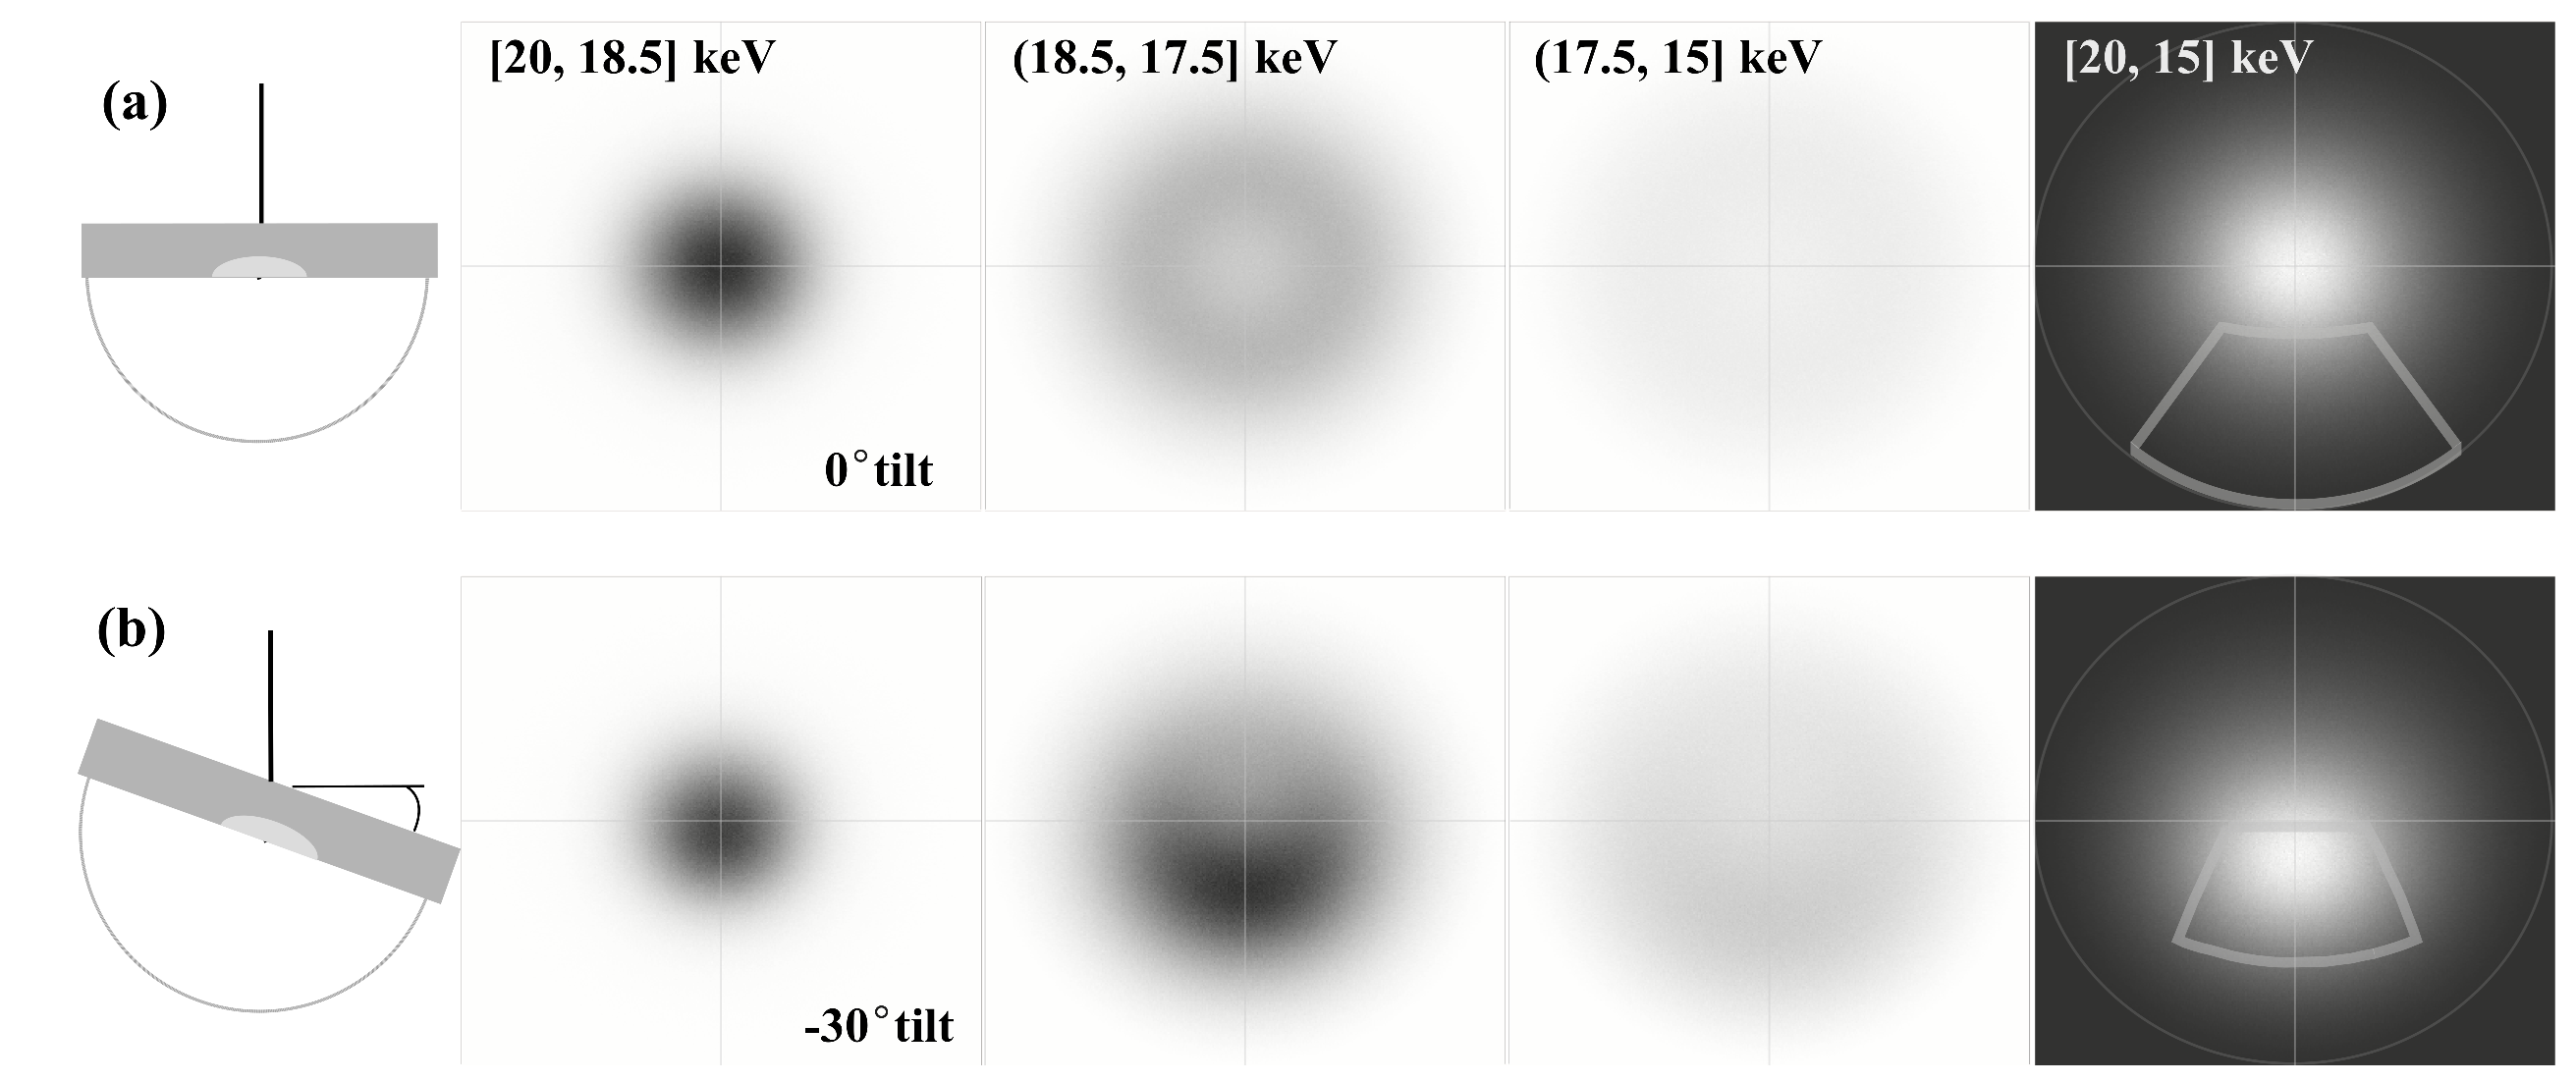
\includegraphics[width=1\linewidth]{Fig1.eps} %TKD_SP_tilt.png
\caption[Directional distributions of transmitted electrons intensity in TKD.]{Directional distributions of transmitted electrons intensity in TKD geometry for two sample tilts (shown in the first column): 0$^{\circ}$~(a) and -30$^{\circ}$~(b). The intensities are shown here as stereographic projections where the intersection of the horizontal and vertical lines indicate the middle of the space (vertical line is the semicircle in the sketch). The first three images in each case are showing  ``energy filtered'' electron intensities (reversed contrast) while the last column displays the total intensity distribution. Image adapted from \cite{PascalTKD}. } 
\label{fig:SP_TKD}
\end{figure}


Fig.~\ref{fig:SP_TKD} (a) shows projections for the case when the sample is horizontal and the electron beam normal. Here we can observe, as expected, that higher energy transmitted electrons are much more focused in the middle of the southern hemisphere, which happens to coincide with the direction of the incident beam. With increased energy loss we can observe an increase in trajectory randomisation or diffuseness. This can be explained by considering the possible trajectories of electrons inside the sample and their corresponding energy loss. Electrons escaping the sample with energies close to the incident beam will not have deviated far from the incident direction. Relative to this, high loss electrons are more likely to escape at large angles to their incident direction. High energy loss electrons appear to have no preferred escape direction and we can expect these electrons to only contribute to image background (FSE2). 

In Fig.~\ref{fig:SP_TKD} (b) we investigate the effect of tilting the sample on the angular distribution of exiting electrons from the bottom surface. Similarly, the high energy electrons will not deviate far from their incident trajectories. However, in this case, the incident direction does not correspond to the centre of the stereographic projection space and we observe that the directional distribution of the low loss electrons clusters  $30^{\circ}$ below the SP horizon. The trajectories of higher loss electrons start to be randomised in the entire SP space. We can also observe in these images how the radial symmetry of electron scattering is broken by the tilt angle of the sample. Finally, the angular distribution of the highest loss electron distribution will look the same as for the flat sample as their ``memory'' of the incident direction is lost.


The outline in the rightmost column of Fig.~\ref{fig:SP_TKD} (a) and (b) depicts a typical detector projected onto the stereographic disk.  The detector has dimensions $24\times 36$ mm$^2$ and is inclined by $10^{\circ}$ from the vertical direction.  The perpendicular distance from the exit point on the bottom of the sample to the detector is $20$ mm, and the top edge of the detector lies in the sample plane for the $0^{\circ}$ orientation.  The detector bottom is closest to the centre of the stereographic projection.  For $0^{\circ}$ sample tilt, most of the scattered electrons miss the detector surface; for a $-30^{\circ}$ sample tilt, the intensity maximum moves upwards onto the lower part of the detector and at the same time the detector projection moves closer to the centre of the stereographic disk, indicating that a significantly larger number of electrons will reach the scintillator.  It should also be noted that a typical raw TKD pattern will display a rather steep intensity gradient from top to bottom, in agreement with the intensity distribution inside the detector outline in Fig.~\ref{fig:SP_TKD} (b) (rightmost image).



It becomes apparent that the sample geometry constitutes an important parameter in the formation of the Kikuchi patterns. Similarly to the EBSD case, where the sample tilt determines the preferred trajectories of electrons of different energies scattering back from the sample~\cite{degraef2013e}, the tilt of the thin film in TKD will directly influence the angular distribution of transmitted electrons suffering diffraction at different energies. In the following section we will carefully review the effect of another system parameter, the sample thickness, on the TKD diffraction patterns. 



\subsection{Non uniform sampled MC}


Joy's Monte Carlo model~\cite{joy1995a}, as described in the previous section, is nothing more than an empirical fit for the energy and direction of backscattered electrons. This, in turn, makes a good start model for the prediction of energy and directions distributions of backscattered electron. The assumption we have made in incorporating the MC model with the dynamical simulations, is that the exit distances of electrons can also be predicted from the MC model. In the absence of a better model it seems adequate to use this approach and experimental results seem to agree to a first approximation~\cite{Deal08}. 

What I want to do in this section is to explore a different approach of sampling the MC predictions of escape distances. I will start by assuming the position in the sample of the primary electrons is  well represented by the elastic events predicted by the MC model. I then run a large MC simulation of electron scattering in a Si sample and store energy, position and direction information for every elastic scattering event. I consider these events my data points.

\begin{figure}[ht]
\centering
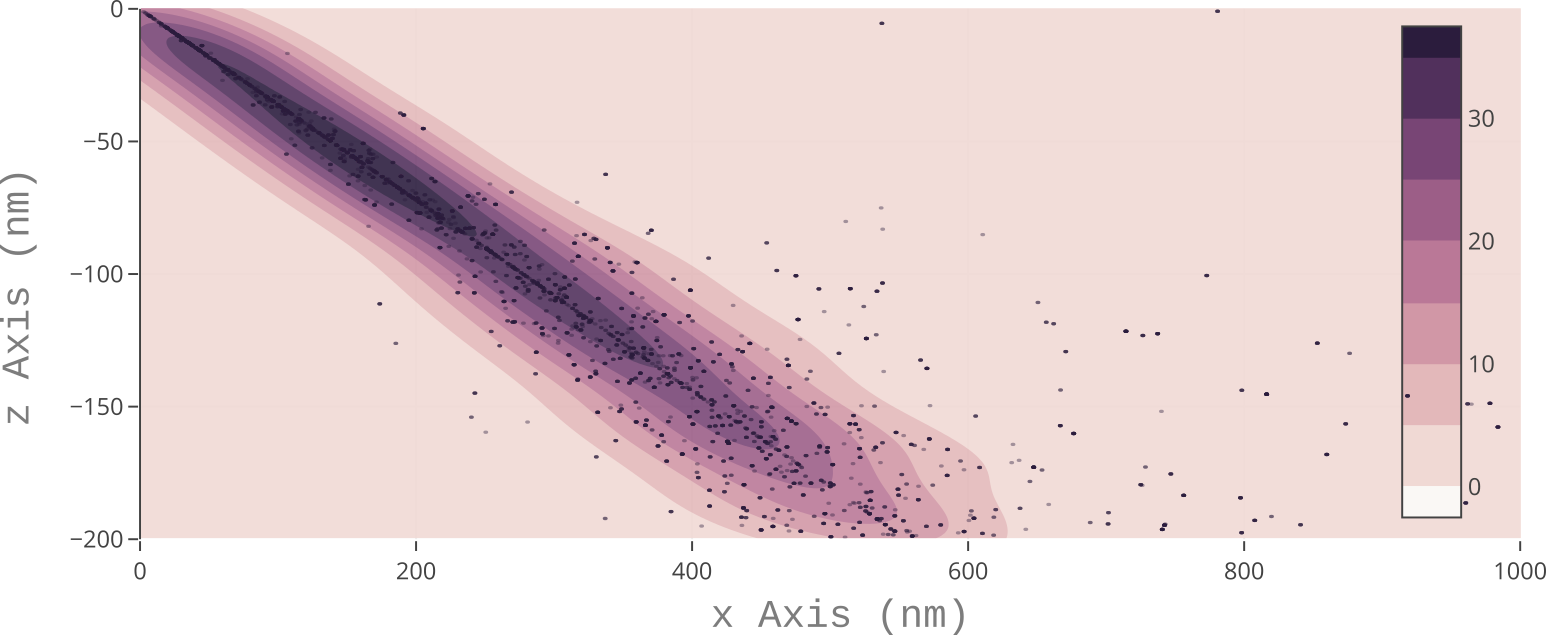
\includegraphics[width=1\linewidth]{Figures/elasticscatter.png}
\caption[Elastic scatter events distribution.]{Visualisation of \SI{10}{\kilo \electronvolt} primary electrons distribution in a Si sample tilted at \SI{70}{\degree}. The scatter points are elastic scattering positions as predicted by the MC model and the pink background is the KDE distribution plot with darker colours indicating higher probability in a linear manner as indicated by the legend in arbitrary units. }
\label{fig:elasticscatter}
\end{figure}

Fig.~\ref{fig:elasticscatter} shows a $xz$ plane projection of primary electron positions. The scatter points plot is made up of random subset of about 1000 points taken from a simulation on 10.000 electrons. The MC simulation used here is the same as described in the previous section. Over-imposed on the scatter plot is a kernel density estimate map using the full data set and showing the areas with highest points density. 




In the following I integrate the KDE map and  use that as a weight in sampling, such that I sample more often from places with more points than from places with fewer points.  The jupyter notebooks \texttt{TKD\_distribution.ipynb} and \texttt{EBSD\_distribution.ipynb} show all the steps described here for sampled MC for a TKD geometry case and a EBSD case, respectively.

I then define the probability of incoherent scattering to be proportional to the distance travelled by the electron until that point. This is in line with the continuous slowing down approximation for inelastic scattering which also scales with travelled distance. Fig.~\ref{fig:incoherentscatter} is showing a weighted sample of 5000 positions and indicates the probability of incoherent scattering with different sized circles.


\begin{figure}[ht]
\centering
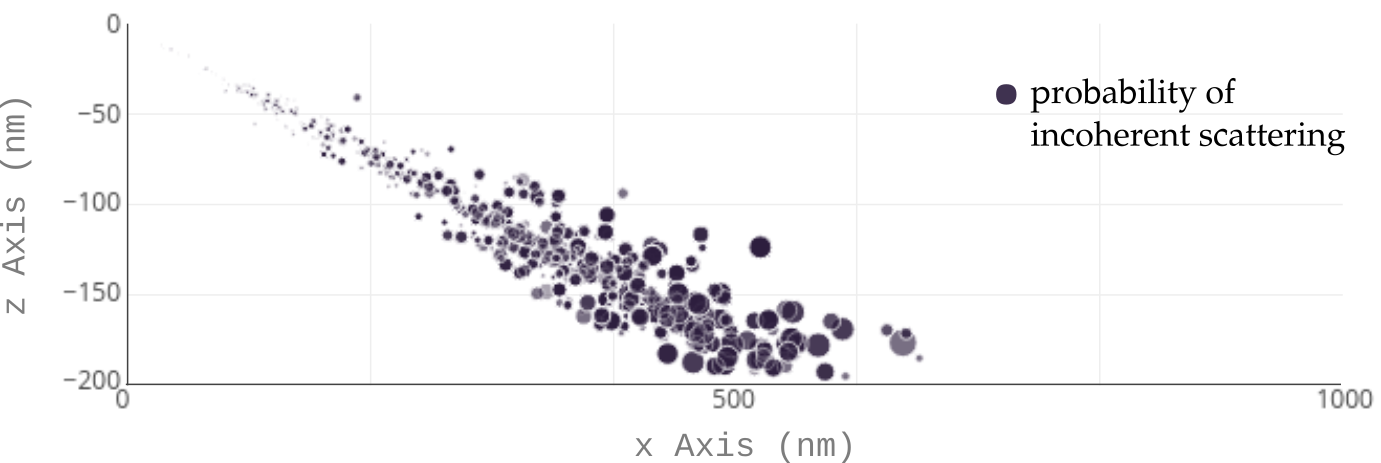
\includegraphics[width=1.\linewidth]{Figures/incoherentscatter.png}
\caption[Incoherent scatter probability.]{Probability of incoherent scattering of primary electrons on their trajectory in the sample. The probability scales with the size of the circle.  }
\label{fig:incoherentscatter}
\end{figure}

Not all these electrons will have the same chance to escape the sample without suffering significant loss of energy. The last bit of weighting that I introduce is an exponential distribution depending on distance to the exiting surface, $z$, where $z$ is taken to be negative. In this case I'm considering the EBSD geometry where the exiting surface is also the entry surface. In effect, the exponential depth weighting is giving more weight to the positions closer to the surface than to those deeper in the sample. This is similar to the weighting factor proposed by Winkelmann \etal for localised BSE~\cite{Winkelmann13}, defined as large angle scattering events followed by less than $n_{ie}$ inelastic events, where $n_{ie}$ is a user defined value.

The last two weighting procedures are competing with each other, the first one favouring data points deeper in the sample and the latter giving more weight to points closer to the surface. This explains why the resulting spatial distribution shown in Fig.~\ref{fig:last_weight} is significantly more localised than the original one in Fig.~\ref{fig:elasticscatter}. More interestingly, it indicates a mean $z$ of about 100-150 nm for 10 keV electrons incident at \SI{70}{\degree} on a Si sample, significantly larger than the original model.  

\begin{figure}[ht]
\centering
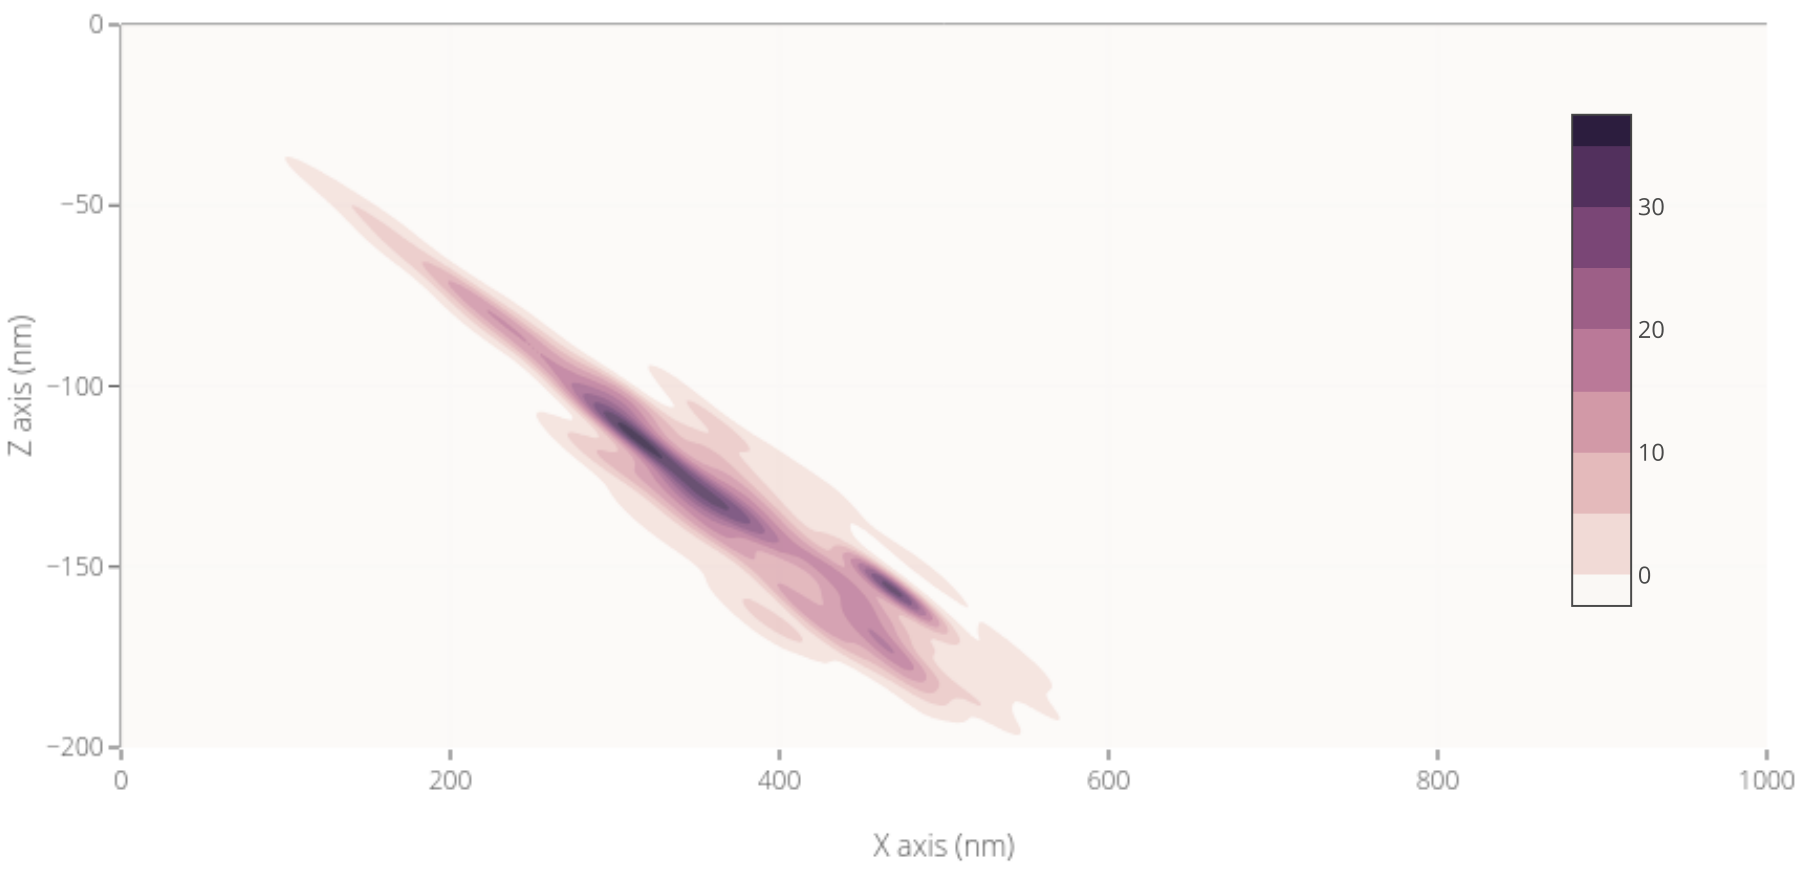
\includegraphics[width=1.\linewidth]{Figures/last_weight.png}
\caption[Estimated spatial distribution of diffraction out ``sources''.]{Estimated spatial distribution of ``sources'' of diffracting out electrons shown as KDE map. Like before, darker colours correspond to higher probability linearly for the colours in the legend.  }
\label{fig:last_weight}
\end{figure}




%
\subsection{Sample thickness in TKD}
\label{sec:TKDthickness}
While for the EBSD and ECP modalities one only needs to run a single Monte Carlo simulation to obtain the energy-depth-direction histogram $\bar{\lambda}_{\mathbf{k}}(E,t)$ for a bulk sample, for the TKD case, the MC simulation results depend on the thickness, $t$, of the sample.
The larger the thickness, the more energy an electron will lose on its way to the exit surface, and this will shift the entire exit energy distribution to lower energies for increasing sample thickness. 




\begin{figure}[ht]
\centering
\includegraphics[width=1.\linewidth]{Fig2.eps}%{Energy_depth_KDE.png}
\caption[KDE plots of electron energy versus escape distance distributions]{KDE plots of electron energy versus escape distance distributions as predicted by the MC model for TKD geometry for two sample thicknesses (a) 100 nm and (b) 200 nm. The area enclosed by the thick line contains 90$\%$ of events. See text for further details. }
\label{fig:E_z_KDE}
\end{figure}

This behaviour is shown in Fig.~\ref{fig:E_z_KDE} as kernel density estimate (KDE) distributions~\cite{KDE} of electron escape energy versus escape distance predicted information for two different Ni thin foil thicknesses, 100 nm and 200 nm respectively, in the TKD geometry. Darker colours show that more electrons are likely to escape the sample with the corresponding parameters. The likelihood  across the two distributions has been normalised to the maximum value in Fig.~\ref{fig:E_z_KDE} (a) such that the intensity across images can be compared. We also show the escape energy and distance region where 90$\%$ of electrons are expected to come from, which is indicated by the thick line. Comparing the two figures, \ref{fig:E_z_KDE} (a) and \ref{fig:E_z_KDE} (b), it is clear that the thickness of the thin sample strongly influences the shape of the distributions. Considering the y-axis, the energy range of the electrons exiting the sample broadens and the energy decreases to significantly lower values as the thickness of the film increases. These observations already indicate that we should expect more diffuse diffraction patterns from thicker samples when compared to thinner ones. In general, the greater the interaction volume of electrons with the sample, the more energy will be lost by electrons before diffraction and the greater the diffuseness of the Kikuchi patterns; as supported by literature~\cite{rice2014}. 

Considering the $x$-axis, we observe that the escape depth profile resembles the usual power-law distribution~\cite{winkelmann2016} with the bulk of the electrons carrying diffraction information originating from a few nm below the escape surface. It should be noted, that the MC model used in this study does not aim to predict the full depth of diffracting electrons or interaction volume. Instead, we make the assumption that the mean value of the full diffraction depth distribution can be estimated to be of the same order as the electron mean free path. Due to the power-law distribution rule, we can be confident that the vast majority of escape depths is considered in this model.

By comparing the two images in Fig.~\ref{fig:E_z_KDE}, we can see that the thickness of the samples impacts very directly the energy distribution of the escaping electrons. This linear correlation is shown more clearly as energy distributions of escaping electrons from a series of different thickness samples in Fig.~\ref{fig:TKDescapeE}. For very thin sample the energy distribution is narrow and we can expect sharp features while for thicker films energy absorption becomes more prominent and distributions will become broader with diffraction lines suffering blurring. The peak of the energy distribution is strongly influenced by sample thickness underlining the requirement for uniform thickness samples in TKD.

\begin{figure}[ht]
\centering
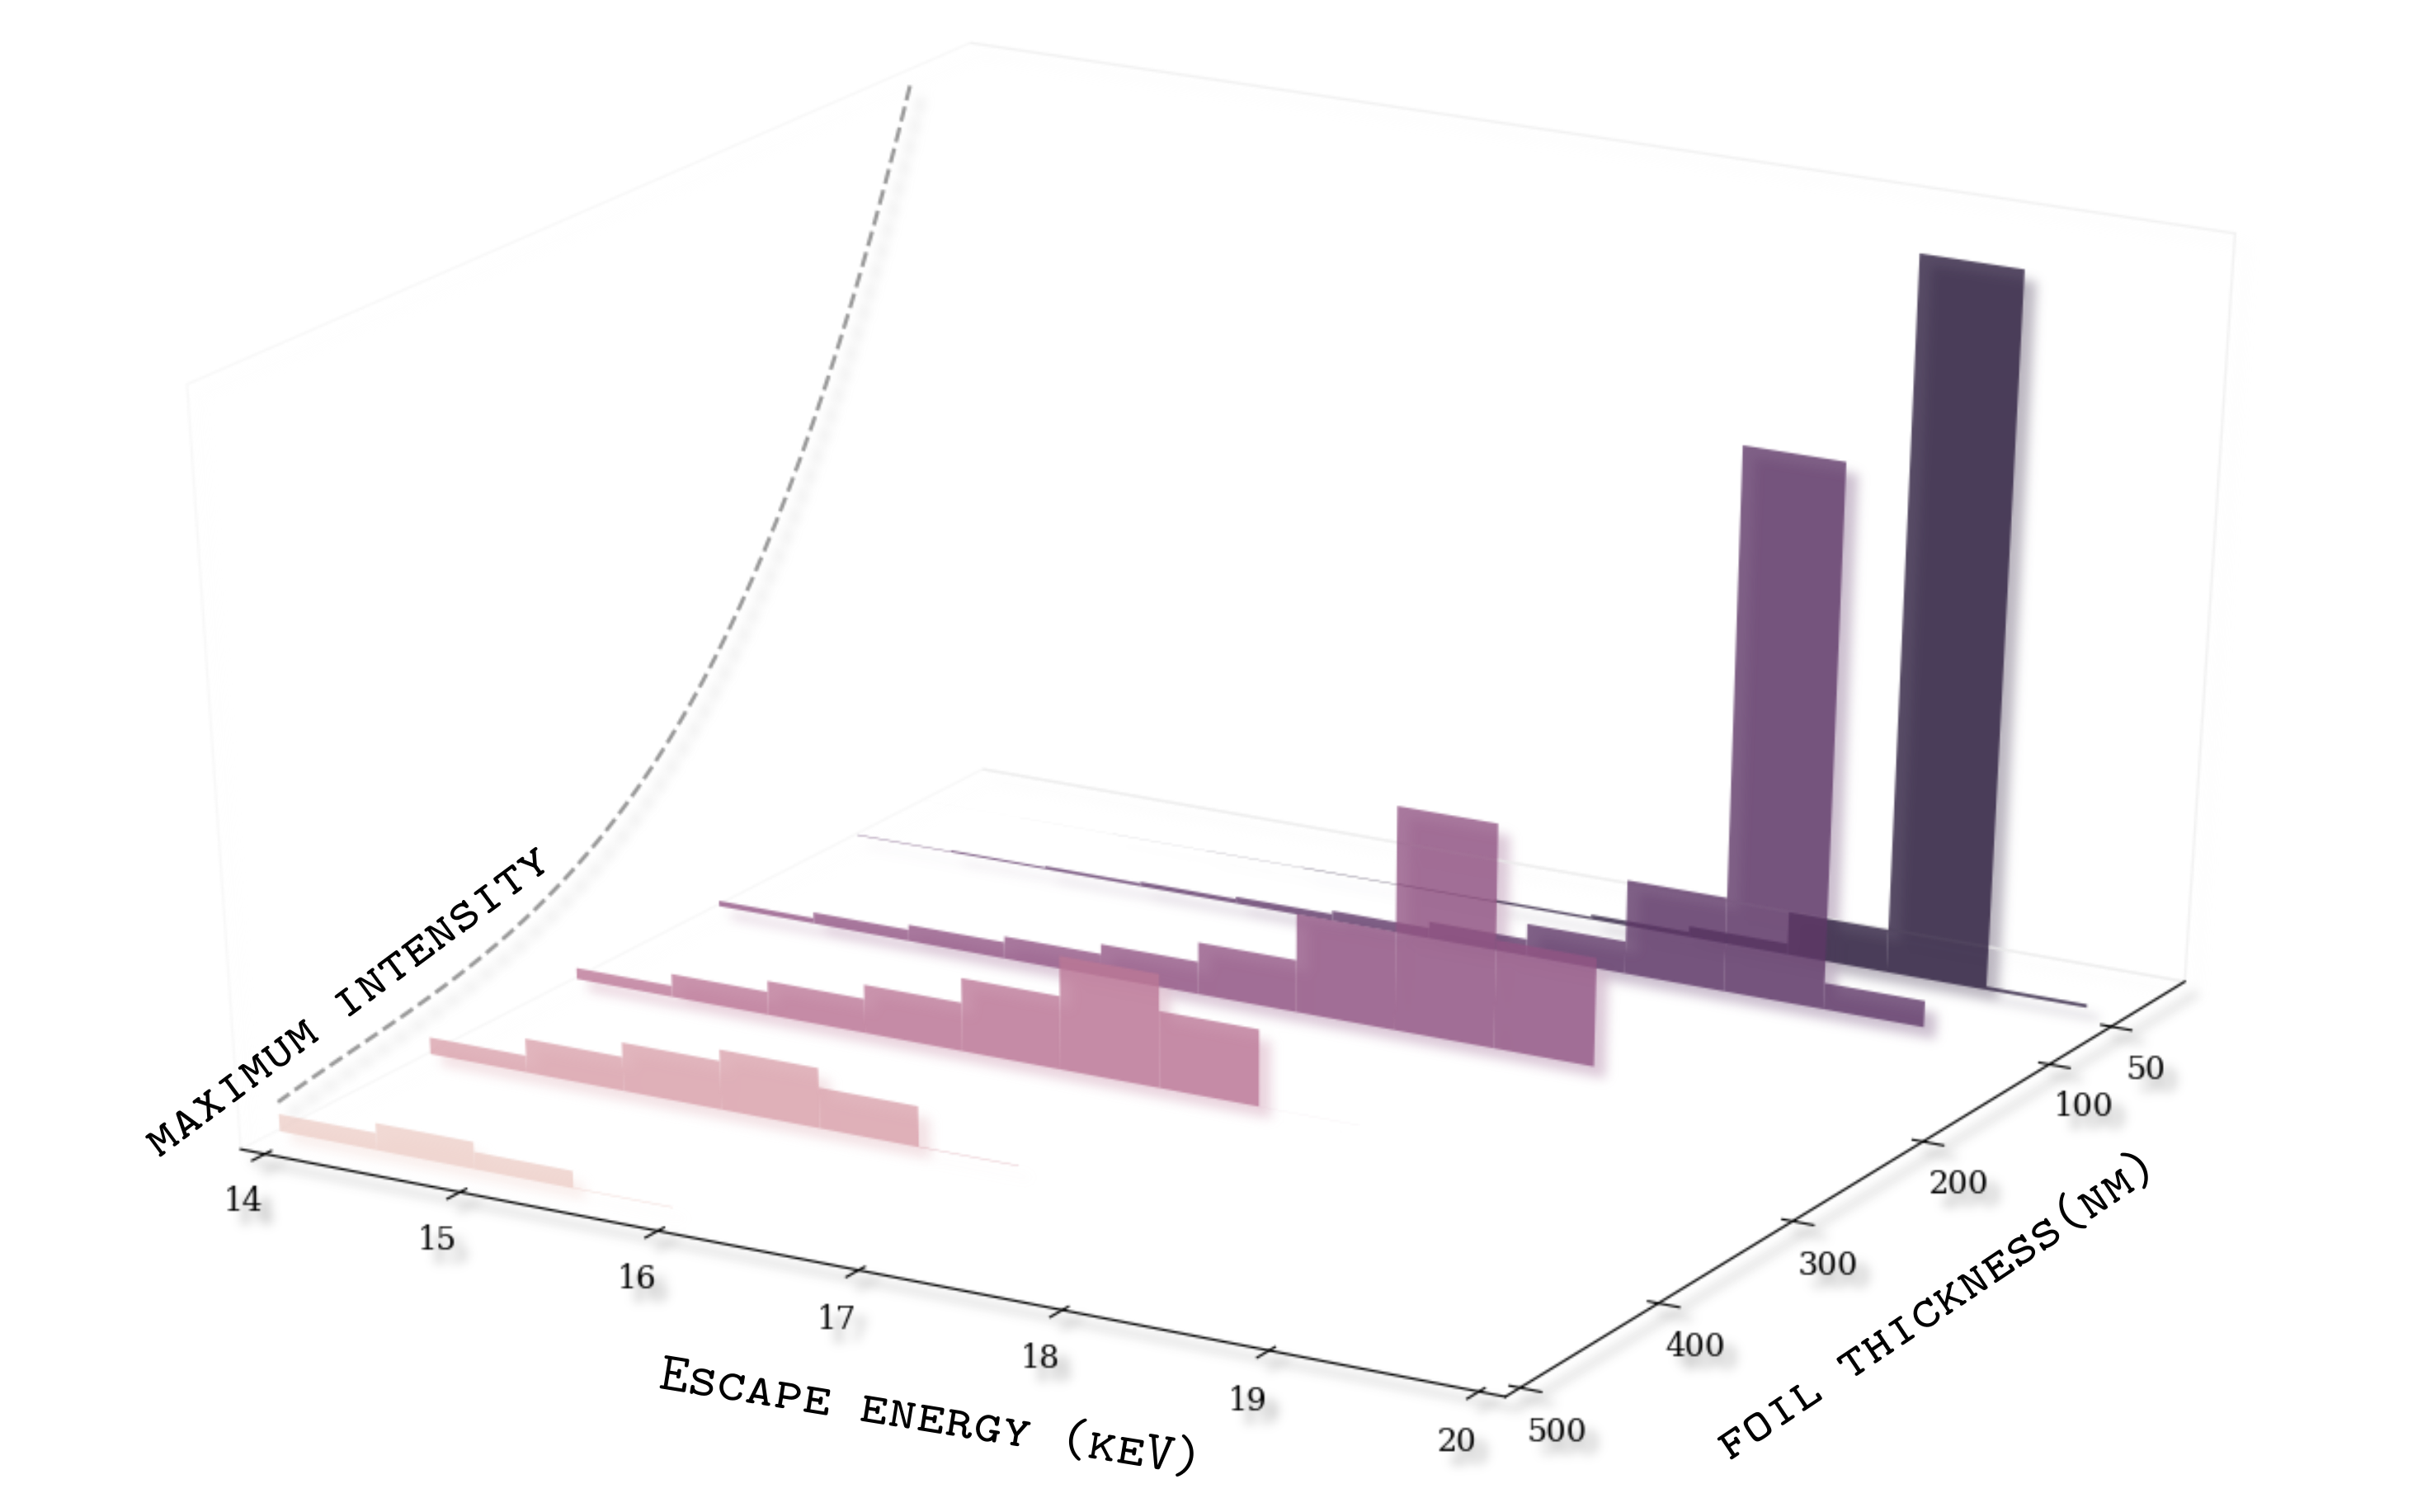
\includegraphics[width=1.\linewidth]{Figures/TKD_escapeE.png}
\caption[Energy distributions versus sample thickness.]{Energy distributions versus sample thickness for electrons exiting a \SI{20}{\degree}  tilted Ni sample for a 20 keV primary beam. Image adapted from \cite{PascalTKD}.  }
\label{fig:TKDescapeE}
\end{figure}



It should be clear that accounting for the effect of sample thickness is essential when predicting accurate electron transmission diffraction patterns. In this model this is achieved by sampling the above likelihood distribution bin-wise and constructing the $\bar{\lambda}_{\mathbf{k}}(E,z)$ weighting function as discussed in Section~\ref{sec:energy_weight} on page~\pageref{sec:energy_weight}.

In the next section, we will investigate special geometries for which electrons reaching different regions of the detector can be described by the same $\lambda_{\hat{\mathbf{k}}}(E,t)$ function, simplifying the calculations significantly. 



%
\subsection{Special sample-detector geometries and the master pattern}
\label{sec:geom}


Let us consider again the sample and detector geometries shown in Fig.~\ref{fig:geometries} (a-f) back on page~\pageref{fig:geometries} where the lighter region on the samples depicts the volume in which electrons suffer scattering events.  Different $\mathbf{k}$ directions are indicated for which energy-distance KDEs distributions are shown in Figure~\ref{fig:ks}.  The top row shows two potential EBSD geometries, one with the sample tilted at the standard $70^{\circ}$ angle with respect to the horizontal plane, the other with the sample tilted at $50^{\circ}$. As previously discussed, the sample geometry will determine the manner in which the radial symmetry of scattering will be broken. Nevertheless, the region of SP space sampled by the position of the detector will also influence the uniformity (or lack thereof) of the electron energies and diffraction distances distributions. In Fig.~\ref{fig:geometries} (a), the electrons that reach the top and bottom of the detector (thick line on the left, inclined at $10^{\circ}$ from vertical) ought to have travelled approximately the same length inside the sample before channelling out; in Fig.~\ref{fig:geometries} (b) on the other hand, the electrons that reach the bottom of the detector have travelled a significantly larger distance inside the sample. 

\begin{figure}[ht]
\centering
\includegraphics[width=1.\linewidth]{Fig4.eps}%{ks_KDEs.png}
\caption[KDE plots of electron energy versus escape distance distributions]{KDE plots of electron energy versus escape distance distributions as predicted by the Monte Carlo model for TKD geometries and directions $\mathbf{k_i}$ shown in Figure~\ref{fig:geometries} (c) and (d). The area enclosed by the thick line contains 90$\%$ of the events.}
\label{fig:ks}
\end{figure}

In TKD, the situation is similar: in Fig.~\ref{fig:geometries} (c) the sample is horizontal and electrons that reach the top of the detector have travelled a much larger distance inside the sample before diffracting than electrons that reach the bottom. In the top row of Fig.~\ref{fig:ks}, the escape energy-escape distance distributions are shown as KDE plots for electrons reaching the top (a) and the bottom (b) of the detector. We can observe qualitative differences in these distributions, especially for the escape energies. The electrons that travelled larger distances before diffracted lost more energy and therefore their energy distribution is shifted towards lower values. On the other hand, a small sample tilt of $-30^{\circ}$ shown in (d) reduces these differences. Fig.~\ref{fig:ks} (bottom row) shows that the energy-distance distribution of electrons reaching the top of the detector (c) and the distribution of those reaching the bottom of the detector (d) is qualitatively the same. Note that figures~\ref{fig:ks} (b), (c) and (d) show similar distributions since all possible trajectories $\mathbf{k_2}$, $\mathbf{k_3}$, $\mathbf{k_4}$ have similar lengths in the sample.

\begin{figure}[ht]
\centering
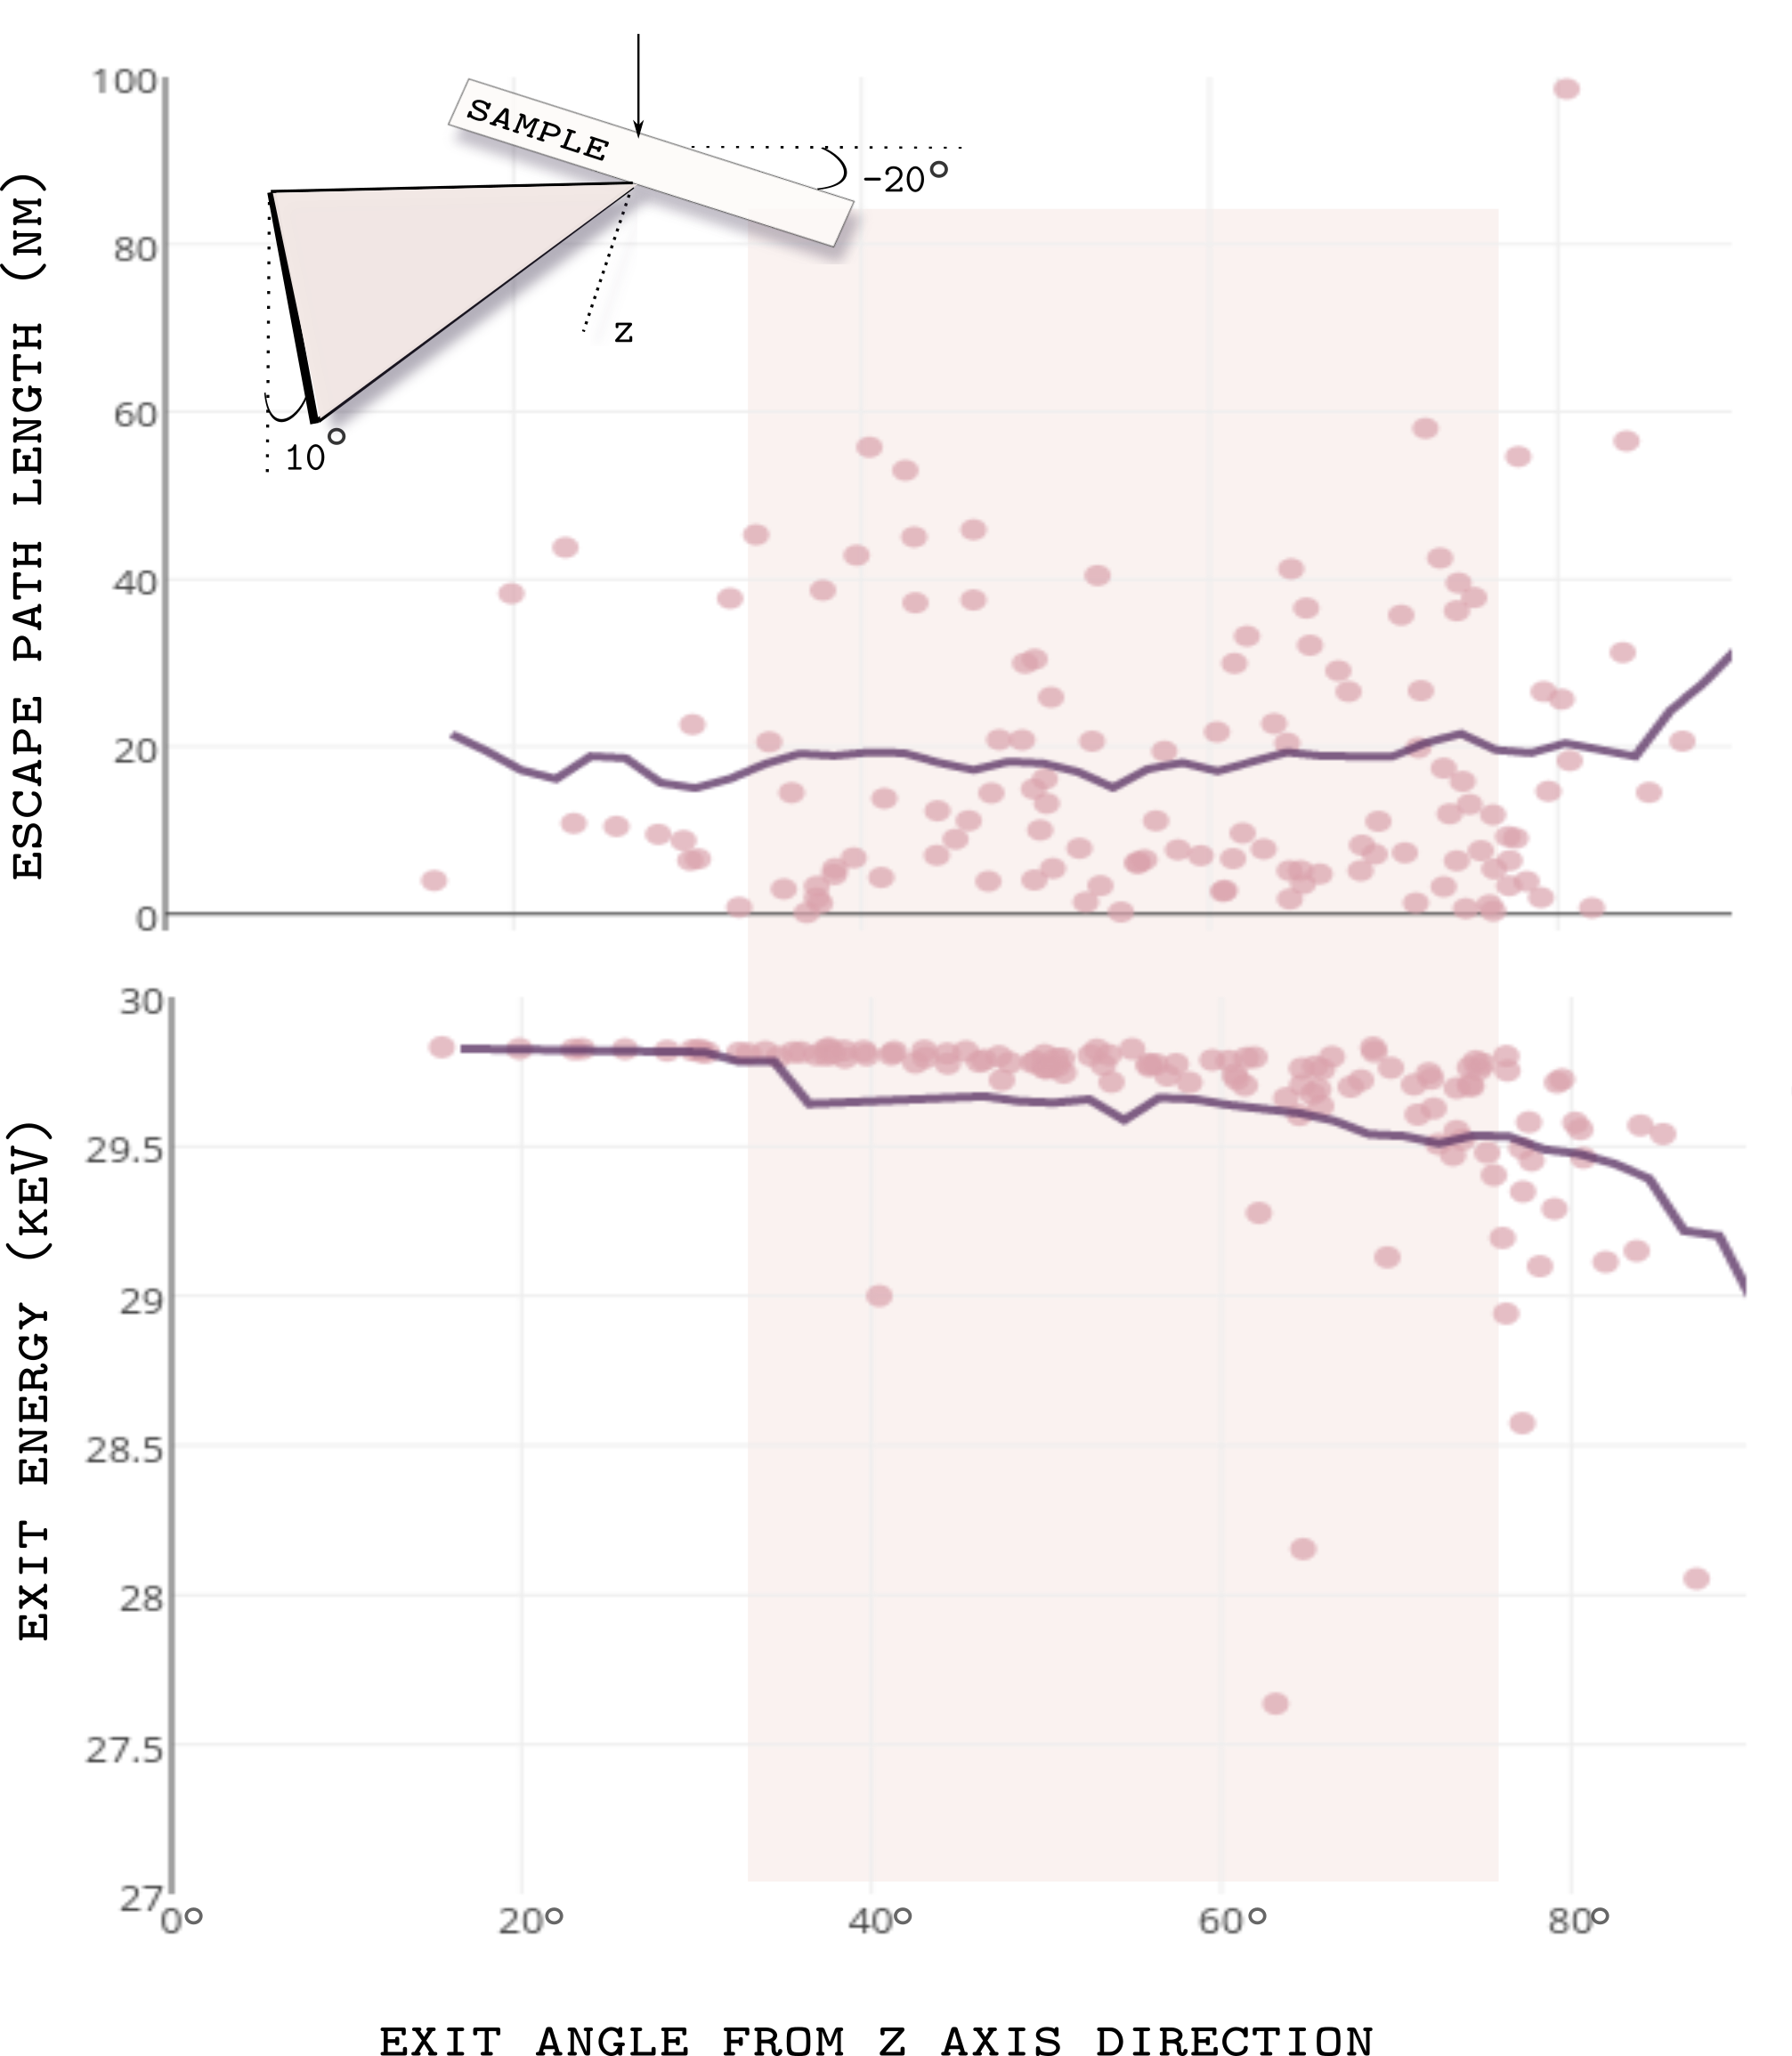
\includegraphics[width=0.8\linewidth]{TKD_angles.png}
\caption[Mean angular dependence of exit energies in TKD]{TKD electron escape path length  (top) and electron exit energy (bottom) dependence on exit angle. Purple line shows the running mean values for more data points than shown. The pink coloured area indicated the solid angle of the detector as shown in the top left insert.}
\label{fig:angles}
\end{figure}


The conclusion we draw here is that in standard TKD geometry the path lengths and energies of electrons that reach the detector do not show strong dependency on the exit angle. To illustrate this even further, in Fig~\ref{fig:angles} I show another, more classical way to show this data, in the form of scatter plot, even though it now contains fewer data points. These are Monte Carlo results for 50000 electrons with incident energy of 30 keV travelling out of a 100 nm Si sample. Note, that I am showing a random sub-sample of 100 points. The angular dependence of both the exit energy (bottom) and the escape path length (top) shows a constant for the predicted solid angle of a detector (between \SI{37}{\degree} and \SI{60}{\degree} from the z-axis direction.) 




Finally, for the ECP case illustrated in Fig.~\ref{fig:geometries} (e) and (f), a small sample tilt does not significantly change the distribution of path lengths inside the sample, and most trajectories have about the same path length. 


This observation has consequences for the numerical approach to be used to obtain high quality simulated patterns. For special geometries, we can now approximate the weighting function $\bar{\lambda}$ by an effective (averaged) weighting function,
\begin{equation}
    \bar{\lambda}_{\hat{\mathbf{k}}}(E,t) \rightarrow \bar{\lambda}(E,t),
\end{equation}
which no longer depends on the electron direction $\mathbf{k}$.  This has significant advantages numerically, since one can now pre-compute the probabilities $P(\mathbf{k})$ for a spherical sampling of incident beam orientations and store the resulting BSE yields in a master pattern (MP) that can be used to generate individual EBSD/TKD patterns by means of bi-linear interpolation, a fast and efficient way to compute many patterns in a short amount of time.  

For EBSD and TKD simulations and sample orientations that deviate significantly from the standard orientations, one cannot apply the above approximation, since the range of distances travelled inside the sample is quite broad; thus, in these cases one must carry out the integrations of Eq.~\ref{eq:Pn} for each individual EBSD/TKD pattern, which results in a slow computational tool.

For ECPs, the situation is quite different, since only BSE1 electrons carry coherent diffraction information; all other (BSE2) electrons only contribute to the background intensity.  A BSE1 electron has nearly the same exit energy as the incident electron since the Rutherford backscatter event is the first major scattering event after entering the sample.  Therefore, nearly all BSE1 electrons have the same exit energy and the energy integration can be eliminated, leading to the following expression which is valid for the ECP case only (with $E_0$ the incident electron energy):
\begin{equation}
    P_n^{\text{ECP}}(\hat{\mathbf{k}}) = \sum_{j\in \mathcal{S}_n}\sigma_j
    \int_0^{t_0(E_0)}\!\!\!\!\!\!\mathrm{d}t\, \bar{\lambda}(t)\vert\Psi_{\hat{\mathbf{k}}}(\mathbf{r}_j;E_0,t)\vert^2,\quad\text{with}\quad  \bar{\lambda}(t) \equiv \frac{\lambda(z)}{N t_0(E_0)}.\label{eq:PnECP}
\end{equation}
Therefore, the master pattern approach is quite well suited for the ECP case as well. For standard geometry EBSD/TKD patterns and ECPs the master pattern is computed only once for a given crystal structure and microscope voltage, and can be used to compute individual patterns by interpolation.  

TKD master pattern simulations proceed along lines similar to the previously published EBSD \cite{degraef2013e} and ECP \cite{degraef2017k} modelling approaches. A uniform grid of points is generated on a spherical surface surrounding a hypothetical spherical crystal located at the centre; each sampling point represents one outgoing beam direction $\mathbf{k}$, and the radius of the sphere is the maximum integration depth $t_0(E)$.  The sampling scheme employs the modified Lambert projection introduced in
\cite{rosca2010a, degraef2013e} in which a uniform grid on a square is mapped onto the sphere by means of an
equal-area projection. For each beam direction, and for a given sample thickness, one carries out the
integrals of equation~\ref{eq:Pn}, using the Monte Carlo $\lambda(E,t)$ weighting function determined for that sample thickness.  In the following section, we show example TKD master patterns and compare them to similar patterns for the EBSD and ECP modalities.



\section{Results}
\subsection{Comparison between EBSD, ECP, and TKD master patterns}
\label{sec:comparison}
The master pattern expression in Eq.~\ref{eq:Pn} reveals that EBSD, ECP, and TKD master patterns have a lot in common; in particular, the dynamical scattering process that underlies the generation of Kikuchi bands is identical for the three diffraction modalities. The only differences occur in the directional, depth, and energy distributions of the B/FSEs that contribute to the patterns.  To illustrate the similarity of the master patterns, Fig.~\ref{fig:MPs} shows a portion of the upper right quadrant (centred on the $[111]$ pole) of the energy-weighted silicon master patterns for (a) ECP, (b) and (c) TKD for two different foil thicknesses ($50$ and $250$ nm) and (d) EBSD. The  microscope voltage is $20$ kV for all patterns, with a specimen tilt angle of $70^{\circ}$ for EBSD, $0^{\circ}$ for ECP, and $-20^{\circ}$ for TKD.  The patterns are very similar but differ in small details. The TKD master patterns are plotted with added colour in order to highlight  subtle differences.

\begin{figure}[ht]
\centering
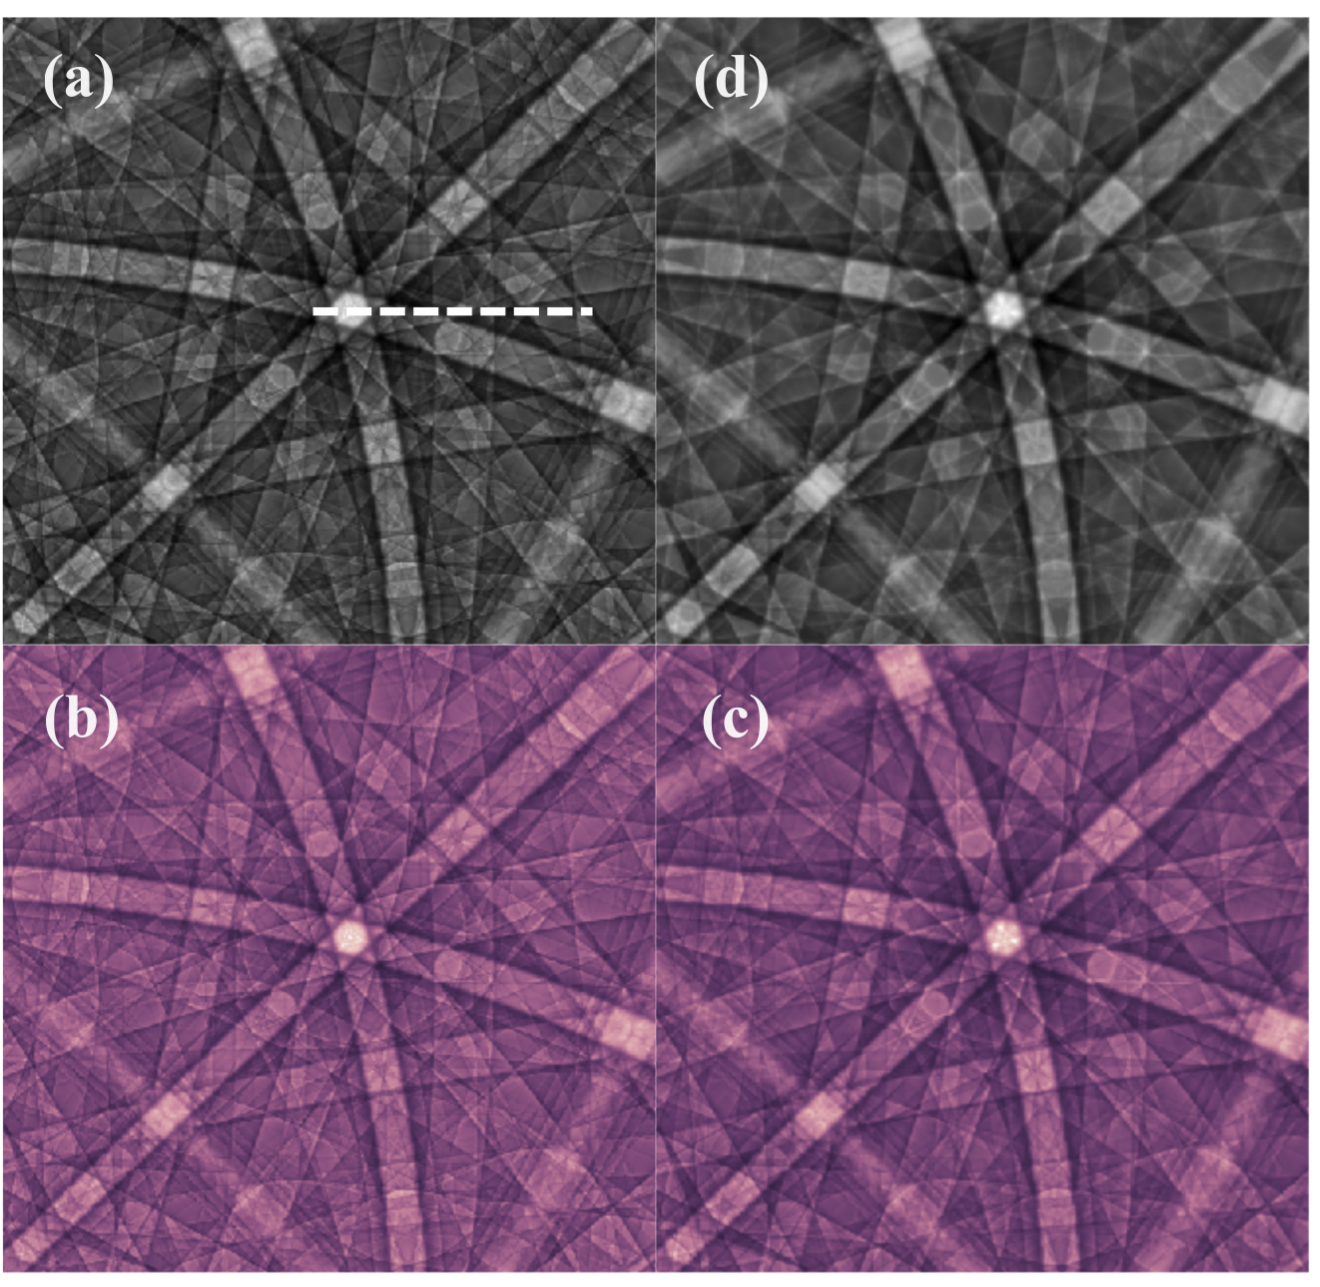
\includegraphics[width=0.9\linewidth]{Fig5a.png}%{MP.png}
\caption[Master patterns for ECP, TKD and EBSD]{Portion of the stereographic projection shown in Fig. \ref{fig:tkspatter}, centred on the $[111]$ pole, of a master pattern for silicon for (a) ECP, (b) and  (c) TKD for sample thicknesses of $50$ and $250$ nm and (d) EBSD.  Image adapted from \cite{PascalTKD}. }
\label{fig:MPs}
\end{figure}


\begin{figure}[ht]
\centering
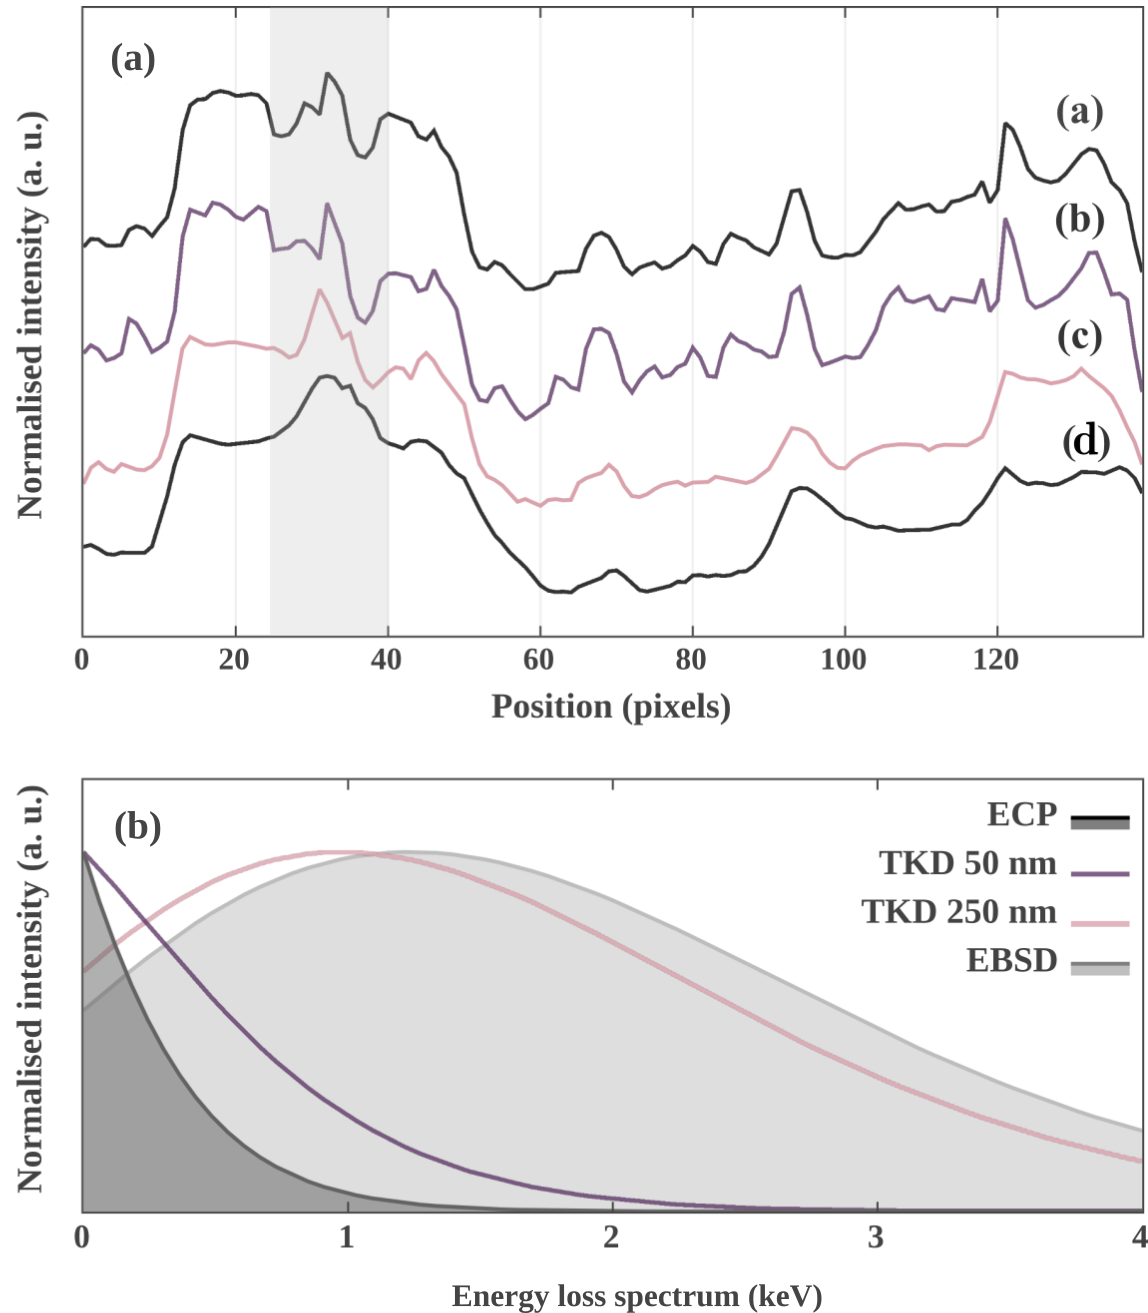
\includegraphics[width=0.7\linewidth]{Fig5b.png}
\caption[Line scans for previous maps and energy distributions]{The profiles in (a) represent the intensity along the central line (marked as a dashed line in Fig. \ref{fig:MPs} (a)), for all four cases; the profiles have been offset vertically for clarity. The energy loss distribution estimated by the MC model for all four cases is shown in (b) as Poisson distribution fitted curves.  Image adapted from \cite{PascalTKD}.}
\label{fig:MPs_lines}
\end{figure}

Fig.~\ref{fig:MPs_lines} (a) shows line scans through each of the master patterns, slightly vertically offset to make the profiles more clearly visible. The differences in details across the patterns is seen here distinctly. The scan across the ECP pattern in Fig.~\ref{fig:MPs} (a) displays significantly better resolved peaks compared to the EBSD one Fig.~\ref{fig:MPs} (d), supporting the better resolution observed in the ECP master pattern. Since the main signal in the ECP case consists of BSE1 electrons which have lost only a small amount of energy in the sample before being backscattered, one can consider ECPs to be energy-filtered versions of EBSPs. 


The line scans across the TKD patterns for different thickness films are more similar to each other, except for the shift in peaks in the zone axis (highlighted by the grey box). It is rather apparent that both the peak positions and the sharpness of the thin film (50~nm) TKD pattern are more similar to the ECP pattern, while the peaks and blurriness of the thick film TKD pattern are closer to those of the EBSPs. In effect, the Master Pattern for TKD on very thin samples is very similar to the ECP MP in similar geometry. If the sample is thicker, the blurriness in the MP for TKD reaches asymptotically the EBSD one. 

We explain this behaviour by considering the energy loss of electrons contributing to the patterns in each case. The Monte Carlo predicted energy loss spectra for all four cases described above are shown in Fig.~\ref{fig:MPs_lines} (b) as fitted Poisson distribution curves. Thin film TKD patterns are produced by electrons with an energy range very close to the ECP case. Similarly, increasing the sample thickness causes the electron exit energy distribution to become wider and shift to lower energies, which corresponds to a broadening and slight blurring of the Kikuchi bands due to the increased Bragg angles; these phenomena are common to EBSPs and thick films TKD patterns. 


It becomes apparent that the sample thickness can be seen as an energy filtering mechanism in TKD as we have seen in Fig.~\ref{fig:TKDescapeE} on page~\pageref{fig:TKDescapeE}. In terms of the traditional Hough-based indexing approach, one must thus select a butterfly mask of the appropriate width, depending on the sample thickness and incident electron energy. For the dictionary indexing approach~\cite{Marquardt17}, used by EMsoft, the pattern dictionary must be computed using the appropriate Monte Carlo and master pattern data, to ensure accurate matches between experimental and simulated patterns.



The EBSD master pattern is an energy-weighted average of individual master patterns and the integration over the electron energy gives rise to a continuous range of Bragg angles and, thus, a general blurring of the master pattern features compared to the ECP case. This will also be the case for individual diffraction patterns that are extracted from the master patterns via bilinear interpolation, as explained in \cite{degraef2013e}.


\subsection{TKD patterns comparison with experiments}

Patrick G. Callahan at University of California, Santa Barbara, acquired a number of experimental TKD patterns, an example of which is shown in Fig.~\ref{fig:TKDpatternfit} a) for a nano-crystalline Aluminum sample, acquired at $30$ kV with a sample tilt of $-18^{\circ}$ in a FEI Teneo field emission scanning electron microscope, using the TSL Hikari EBSD detector system.  The sample foil is approximately $150$ nm thick.  The calibration parameters are given in Table \ref{Table:calParams}. I added axes showing the radial distance components from the pattern centre, $r_x$ and $r_y$, respectively :

\begin{align*}
    r_x &= tan(\theta_x) = \frac{(x - x_{PC}) \rho}{L} \\ 
    r_y &= tan(\theta_y) = \frac{(y - y_{PC}) \rho}{L}
\end{align*}


\begin{table}
    \centering
    \begin{tabular}{l l l l }
    \toprule
    $x_{PC}$ (pixels) & $y_{PC}$ (pixels) & $\rho$ (\si{\micro \meter}/pixel) & $L$ (\si{\micro \meter})\\
    \midrule
     6.4406 & 264.1950 & 0.292 & 23471.48 \\
    \bottomrule     
    \end{tabular}
    \caption[Calibration parameters.]{Pattern centre position $(x_{PC}, y_{PC})$ (given in the reference frame of the detector with origin in the middle as shown in Fig. \ref{fig:TKDgeometry}), detector pixel size $\rho$ and distance from sample to detector $L$  for the TKD pattern shown in Fig. \ref{fig:TKDpatternfit}. }
    \label{Table:calParams}
\end{table}



\begin{figure}[ht]
\centering
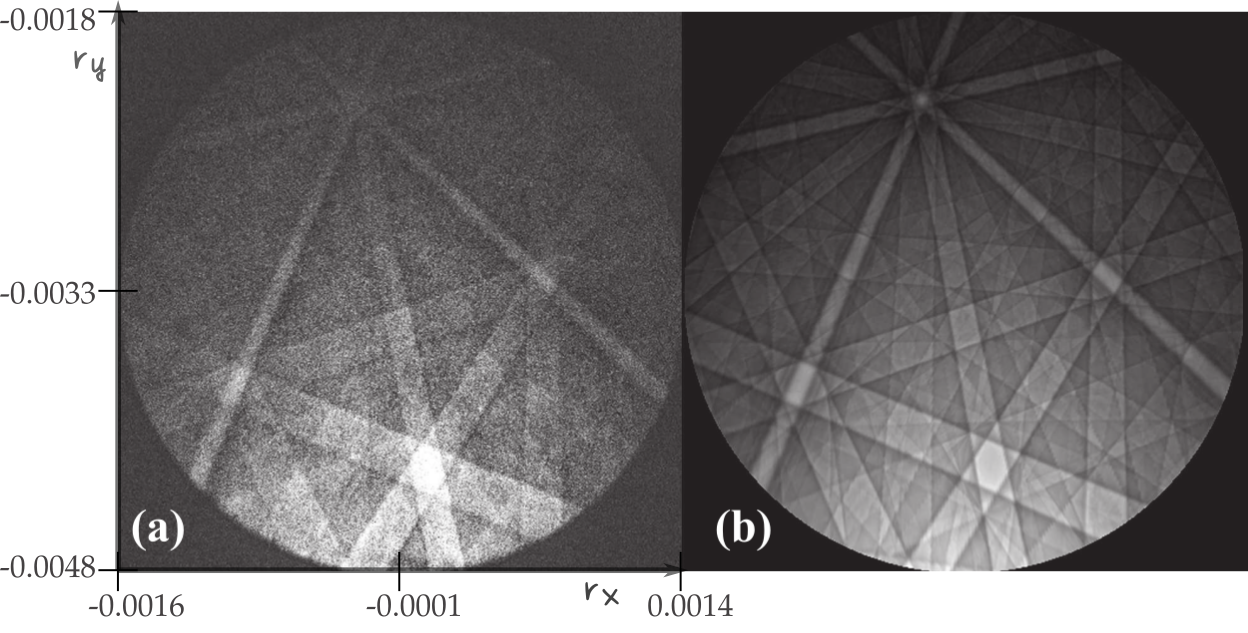
\includegraphics[width=1.\linewidth]{Fig6.png}
\caption[Experimental TKD patterns.]{(a) Experimental TKD patterns for Al at $30$ keV; brightness and contrast of the simulated patterns have been adjusted to better match the experimental patterns. The axes are showing the radial distance components from the pattern centre $r_x$ and $r_y$. (b) Corresponding simulated patterns. Image adapted from \cite{PascalTKD}. }
\label{fig:TKDpatternfit}
\end{figure}

Fig.~\ref{fig:TKDpatternfit} b) shows the dictionary indexing simulations with this model and we can see that it matches the experimental patterns well. The dot product values between normalised patterns are equal to $0.881$ which indicates a satisfactory match. For more details about the parameters that go into the simulation see the paper~\cite{PascalTKD}.

Note that the only adjustments to the simulated patterns were brightness and contrast changes to maximise the visual agreement between the simulated and experimental patterns.  The overall intensity gradient (from bright at the bottom of the pattern to dark at the top) follows directly from the use of the direction-dependent Monte Carlo statistical data, and is in good agreement with the intensity gradients of the experimental patterns.  The satisfactory agreement between simulated and experimental patterns indicates that the energy-weighted dynamical scattering model employed in the pattern simulations is sufficient to obtain realistic pattern simulations. 

Next, he generated a TKD master pattern with the energy filtering model for an Al sample as shown in the paper. For all of the experimental patterns  of an acquired TKD map of a nano-crystalline Al sample  the dictionary indexing approach finds the simulated patterns from the MP that best matches it. 

Fig.~\ref{fig:TKDindex}~a) shows an orientation similarity map. The dictionary indexing approach produces a list of the top N best matches (dictionary patterns with the N highest dot products, where N is typically set to 30). For each sampling point, the orientation similarity is computed by determining the average number of top matches that this sampling point has in common with its four nearest neighbours; this value is then displayed as a grey scale image. Since sampling points near grain boundaries will have fewer best matches in common with their neighbours, the orientation similarity map (OSM) provides an easy overview of the microstructure in which grain interiors have a uniform intensity level and all grain boundaries have lower intensity.

The \hkl[010] inverse pole figures in Fig.~\ref{fig:TKDindex}~b) and c) were obtained by the standard commercial OIM-8 indexing package and the dictionary indexing approach, respectively. The dark regions near the top of the field of view in Fig.~\ref{fig:TKDindex}~b) correspond to surface contamination from the XeF2 etching step and result in clusters of incorrectly indexed or unindexable points in both indexing approaches; patterns were deemed to be unindexable when the Image Quality was low (according to the commercial software analysis package). However, overall, the dictionary indexing approach with the energy-weighted model has fewer undindexable or incorrectly indexed points, in particular near grain boundaries.

\begin{figure}[t]
\centering
\includegraphics[width=1.\linewidth]{Fig7b.png}
\caption[Dictionary indexing TKD pattern]{ (a) Orientation similarity map (see text for details); (b) [010] inverse pole figure (IPF) obtained with the commercial OIM-8 indexing software; and (c) [010] IPF obtained using the dictionary indexing approach. Image adapted from \cite{PascalTKD}. }
\label{fig:TKDindex}
\end{figure}



%
\section{Discussion and conclusions \label{sec:discussion}}

Inelastic scattering, a phenomenon usually discarded in diffraction simulations, has direct influence on the energy distribution of diffracting electrons and, consequently, on the imaged Kikuchi patterns. The broader the energy distribution of diffracting electrons, the more diffuse the Kikuchi band edges. Using a Monte Carlo model we can observe that the length of electron trajectories before diffraction is a determining factor in the broadening of the energy distribution. This factor, in turn, can be controlled in the Transmission Kikuchi Diffraction modality through the thickness of the sample, acting effectively as an energy-filtering mechanism. Another determining factor for the energy distribution is the sample-detector geometry which influences both TKD and EBSD modalities.



We should note that the Monte Carlo model used in this work explicitly describes the lower escape distance values for the signal carrying electrons.  A subset of electrons reaching the detector will, nevertheless, carry a probability of channelling over longer trajectories. Depending on their travel direction inside the crystal, these electrons are expected to give rise to contrast inversion of one or more Kikuchi bands (observed as dark instead of bright lines). This will occur when the distance travelled is of the order of, or larger than, the extinction distance for a particular plane. Contrast inversions are thus expected to occur for both EBSD and TKD modalities when the sample is tilted such that long electron trajectories are possible; in addition, the sample should have a crystal structure that gives rise to short extinction distances. For the ECP modality, contrast inversions are not expected to occur unless very large sample tilt angles are used, which is not practical due to the possibility of the sample hitting the back-scatter detector. Similarly, when the TKD detector if mounted horizontally, below the sample, the electron trajectories inside the sample will have a narrow range of escape distances, so that contrast inversions are also not expected to occur. A statistical model more sensitive to the outlier cases of long distance channelling electrons is therefore necessary if we are to correctly predict band contrast inversion. 

The energy-weighted scattering model is shown to correctly predict Kikuchi bands sharpness (defined as signal to noise intensity) for the different SEM modalities. When used for the dictionary indexing approach it was shown to produce indexed TKD patterns with fewer incorrectly indexed points compared to commercial Hough transform based indexing software. 
